\chapter{Effective Theory of Preactivations at Initialization}\label{ch:signalprop}
\label{ch:eft-mlp}


\epigraph{We believe this realm of work to be immensely important and rich, but we expect its growth to require a degree of critical analysis that its more romantic advocates have always been reluctant to pursue \dots.}{
Minsky\index{Minsky, Marvin} and 
Papert\index{Papert, Seymour} in the prologue to their 1988 expanded edition of \emph{Perceptrons} \cite{miskypapertperceptron}.}





\noindent{}The key defining feature of \terminate{deep learning} is the stacking of components on top of each other in order to get a \emph{deep} \terminate{neural network} \terminate{architecture}.
Despite the empirical preference for deeper networks, it's not at all obvious \emph{why} deep is good for learning. For a fixed number of neurons per layer, deep implies many more parameters, and often in deep learning more parameters lead to better performance. But there are other ways to include more parameters. For instance, why not just have a single hidden layer that is very wide?
In fact, in the strict infinite-width limit, such a single-layer model has the same number of parameters as any deeper MLP: infinity.

The proper way to think about the effects of depth is not to just count the number of model parameters, but instead to ask what happens when we add an additional layer to our MLP. In~\S\ref{ch:ngp}, we developed a formalism to address exactly this question through recursions for observable quantities of interest, enabling us to compute how the distributions of initial network outputs change upon adding a layer.
What we need, then, is a tool to effectively extract the explicit depth dependence from these recursions.



Building on the effective theory formalism developed in~\S\ref{ch:ngp}, in this chapter we'll extend the criticality and fluctuation analyses performed in~\S\ref{ch:deep-linear-eft} to MLPs with any nonlinear activation function.
Enlightened by the success of the previous chapter in finding simplification in the wide regime ($n \gg 1$), we now seek additional simplicity in the limit of large depth ($L \gg 1$).\footnote{What this means -- in light of the discussion in \S\ref{sec:solution_DLN} -- is that we take the limit of large width \emph{first} and then look at the limit of large depth.}
We'll first analyze the limit of infinite number of neurons per layer,
and then back off this limit to consider networks of large but finite width and depth. The result will be explicit expressions for the two-point and four-point correlators of preactivations in these asymptotic limits.\footnote{Despite the asymptotic nature of these solutions, we note many of these tools were developed to study the strong interactions, where a parameter that is $3$ in practice is taken to be infinity. Thus, sometimes even $3 \sim \infty$, since $1/3 \ll 1$ can be made to work as perturbative parameter \cite{Coleman:1985rnk}.
}

This will let us address the question of what happens to input signals as they propagate through the many layers of deep neural networks at initialization (\S\ref{sec:bootstrapping}).
We'll come to understand that the order-one values of the \terminate{initialization hyperparameters} -- i.e.~the bias variances $\Cb{\ell}$ and the rescaled weight variances $\CW{\ell}$ -- have pronounced qualitative effects on the behavior of the observables, just as we saw in \S\ref{ch:deep-linear-eft} for deep linear networks.
In particular, we'll explain how neural-network behavior becomes increasingly sensitive to these \terminate{initialization hyperparameters} with increasing depth.\footnote{The initial part of this analysis  was first carried out in a series of papers, \cite{poole2016exponential,raghu2017expressive,schoenholz2016deep}, using a different set of techniques that are ultimately equivalent to ours in the infinite-width limit.  Extending this analysis, we'll identify two very general  conditions according to the \emph{principle of criticality}\index{criticality!principle of} that let us determine the correct order-one values for the initialization hyperparameters.
In \S\ref{sec:generalization-at-infinity}, we'll see that the need for these conditions can also be understood by demanding that fully-trained networks generalize well. 
}

Such a tuning brings a network to \neo{criticality}, a term we borrow from statistical physics used to describe self-similar systems.
To this end, we give a general prescription for tuning \terminate{initialization hyperparameters} to their critical values for a given activation function and network architecture (\S\ref{sec:scale-invariant-eft} and~\S\ref{sec:non-scale-invariant-eft}). In the process, we also identify some activation functions that don't allow for criticality.
We will also see that certain activation functions behave very similarly to each other when tuned to criticality, highlighting an important connection to the notion of \neo{universality} in statistical physics.\index{statistical physics}

\index{effective theory of deep learning}
The study of finite-width corrections at criticality then leads us to one of the main results of this chapter, an \neo{emergent scale} given by the aspect ratio of the network depth to the network width, $L/n$ (\S\ref{sec:signal_prop_finite_width}).
This aspect ratio ultimately
serves as the 
\emph{cutoff}\index{cutoff, effective theory} of our effective theory, %
controlling the region of validity of our effective theory as well as determining the strength and importance of the finite-width corrections to the infinite-width description.
On the one end of the spectrum, we find that the shorter and fatter networks are, the more and more that they behave like their infinite-width counterparts. 
On the other end, skinny and tall networks become increasingly dominated by non-Gaussian \neo{fluctuations} due to \neo{interactions} between neurons. Overall, this serves to generalize our fluctuation analysis for deep linear networks\index{deep linear network} in \S\ref{sec:fluctuations_DLN}.


Lastly, we'll  conclude the chapter by addressing and resolving a subtlety that arises in our criticality analysis for non-smooth activation functions such as the $\relu$ (\S\ref{sec:finite_angle}).








































\section{Criticality Analysis of the Kernel}\label{sec:bootstrapping}
For the bulk of this chapter, our goal is to extend the notion of criticality discussed in~\S\ref{ch:deep-linear-eft} to deep MLPs with general activation functions $\sigma(z)$. Our starting point is the kernel recursion
\be\label{eq:kernel-recursion-reminder}
\Ti{\ker}{\alpha\beta}{\ell+1} = C_b + C_W \braket{\sigma_{\alpha}\sigma_{\beta}}{\ell} \, ,
\ee
derived in the previous chapter. %
As a reminder,
the \neo{kernel} $\Ti{\ker}{\alpha\beta}{\ell}$, defined by~\eqref{eq:leading-kernel-reminder}, is the infinite-width limit of the mean metric $\Ti{G}{\alpha\beta}{\ell}$. Here, in order to restrict the number of distinct hyperparameters, we have set the bias variance $C_b^{(\ell)}=C_b$ and the rescaled weight variance $C_W^{(\ell)}=C_W$ to be layer-independent.
The initial condition for this recursion is given by the first-layer kernel %
\be\label{eq:kernel-initial-condition}
\Ti{\ker}{\alpha\beta}{1}=C_b+C_W\!\le(\frac{1}{n_0}\sum_{i=1}^{n_0}\x{i}{\alpha}\x{i}{\beta}\ri)\, ,
\ee 
set by the inner products of inputs $\sum_{i=1}^{n_0} \x{i}{\alpha}\x{i}{\beta}$. Our goal is to analyze how the kernel changes as a function of layer and, as we'll see, this analysis at the level of the kernel is sufficient to pin down the critical initialization hyperparameters to leading order in $1/\text{width}$.\index{initialization hyperparameters!critical}


For deep linear networks\index{deep linear network}, the Gaussian expectation of the activations  with respect to the kernel is just given by the kernel, $\braket{\sigma_{\alpha}\sigma_{\beta}}{\ell}=\braket{z_{\alpha}z_{\beta}}{\ell}=\Ti{\ker}{\alpha\beta}{\ell}$, and the recursion equation was simple enough for us to obtain a full solution. Stepping outside the realm of the $\linear$ activation function, however, the kernel recursion acquires two new complications that require some care: (i) the expectation value $\braket{\sigma_{\alpha}\sigma_{\beta}}{\ell}$ will be a nonlinear function of the kernel, and (ii) for two distinct inputs $\alpha\ne\beta$ the recursion mixes off-diagonal components $\Ti{\ker}{\alpha\beta}{\ell}$ with diagonal components $\Ti{\ker}{\alpha\alpha}{\ell}$ and $\Ti{\ker}{\beta\beta}{\ell}$.

\index{activation function!quadratic@\texttt{quadratic}}
Let's illustrate this with a $\texttt{quadratic}$ activation function $\sigma(z)=z^2$. 
As should be second nature by now, evaluating \eqref{eq:kernel-recursion-reminder} requires two pairs of Wick contractions\index{Wick contraction}, giving
\begin{align}
\Ti{\ker}{\alpha\beta}{\ell+1} &= C_b + C_W \braket{z_{\alpha}^2 z_{\beta}^2}{\ell} \,  \\
&=C_b+C_W \le(\Ti{\ker}{\alpha\alpha}{\ell}\Ti{\ker}{\beta\beta}{\ell}+2\Ti{\ker}{\alpha\beta}{\ell}\Ti{\ker}{\alpha\beta}{\ell}\ri)\, .\nonumber
\end{align}
Thus, unlike deep linear networks\index{deep linear network}, for quadratic activations $\Ti{\ker}{\alpha\beta}{\ell+1}$ depends not only on $\Ti{\ker}{\alpha\beta}{\ell}$ but also on $\Ti{\ker}{\alpha\alpha}{\ell}$ and $\Ti{\ker}{\beta\beta}{\ell}$, requiring us to solve three coupled nonlinear recursion equations for $\alpha\ne\beta$.
This mixing is generic for nonlinear activation functions.

 

For practitioners, this is good news: the off-diagonal elements of the kernel are related to the generalization ability of the network. For deep linear networks\index{deep linear network} the lack of mixing via nonlinearity suggests an \neo{inductive bias} that limits such networks' ability to develop nontrivial correlations for pairs of samples. %
While mixing is a benefit in practice, it's an obstacle in theory, albeit a surmountable one. Since the kernel recursion mixes at most two inputs, it is sufficient to analyze the case with a single input and the case with two distinct inputs. We shall now perform these analyses in turn, with an eye towards deriving the general conditions for criticality.




\subsubsection{A single input}
Each diagonal component of the kernel can be solved self-consistently by itself. Specifically, labeling a single input by $\alpha=\M$,
\begin{align}\label{eq:kernel-diagonal}
\Ti{\ker}{\M\M}{\ell+1}& = C_b + C_W\braket{\sigma(z_{\M})\,\sigma(z_{\M})}{\ell} \,  \\
&=C_b + C_W g\!\le(\Ti{\ker}{\M\M}{\ell}\ri) \, . \nonumber
\end{align}
Here, we introduced a helper function
\be\label{eq:helper_first}
g\!\le(K\ri)\equiv \le\langle \sigma(z)\, \sigma(z)\ri\rangle_{K} \equiv \frac{1}{\sqrt{2\pi\ker}} \int_{-\infty}^{\infty}d z\  e^{-\frac{z^2}{2\ker}}\, \sigma(z)\, \sigma(z)  \, ,
\ee
to emphasize that the expectation $\braket{\sigma(z_{\M})\sigma(z_{\M})}{\ell}$ is a function only of a single component of the kernel, $\Ti{\ker}{\M\M}{\ell}$.
By focusing our attention first on the single-input kernel, we can deal with the nonlinearity before confronting the mixing of kernel components.

\index{fixed point!trivial}
In particular, the single-input recursion~\eqref{eq:kernel-diagonal} is really telling us how the average magnitude of the preactivations for the input
\be\label{eq:midpoint-kernel-def}
\Ti{\ker}{\M\M}{\ell} = \mathbb{E}\le[\frac{1}{n_{\ell}}\sum_{i=1}^{n_{\ell}}\le(\z{i}{\M}{\ell}\ri)^2\ri]\, ,
\ee
changes as a function of layer $\ell$, with the initial condition for the recursion set by \eqref{eq:kernel-initial-condition}.
For the same reasons we considered in~\S\ref{sec:criticality_DLN}, we would like that the kernel $\Ti{\ker}{\M\M}{\ell}$ neither exponentially explode nor exponentially vanish.
However, such exponential behavior is generic, and so for most choices of initialization hyperparameters $\le(C_b,C_W\ri)$, the kernel will either explode exponentially towards a \emph{trivial} fixed point at infinity or collapse exponentially onto a trivial fixed point at a finite value $\Tif{\ker}{\M\M}$. Thus, our first \terminate{criticality} condition is to mitigate this exploding or collapsing kernel problem for the single input.\index{exploding and vanishing kernel problem}


There is an ancient technique used to analyze nonlinear recursions such as the single-input kernel recursion~\eqref{eq:kernel-diagonal}: linearization around a fixed point.
Namely,
we first identify a fixed point of the recursion, i.e.~a value $\Tif{\ker}{\M\M}$ that satisfies
\be\label{eq:fixed_single}
\Tif{\ker}{\M\M}=C_b + C_W g\!\le(\Tif{\ker}{\M\M}\ri)\, ,
\ee
and then expand the kernel around it as 
\be\label{eq:fixed-point-expansion-Delta-K}
\KML=\Tif{\ker}{\M\M}+\Delta \KML. 
\ee
This expansion for the single-input recursion~\eqref{eq:kernel-diagonal} results in the linearized recursion
\be\label{eq:single_expand}\index{kernel!linearized recursion}
\Ti{\Delta \ker}{\M\M}{\ell+1}=\chi_{\parallel}\!\le(\Tif{\ker}{\M\M}\ri)\Ti{\Delta \ker}{\M\M}{\ell}+O\!\le(\Delta^2\ri)\, , %
\ee
where we introduced the \term{parallel susceptibility}\index{susceptibility!parallel|see{parallel susceptibility}}\index{susceptibility!perpendicular|see{perpendicular susceptibility}}
\begin{align}\label{eq:chi_parallel_first}
\chi_{\parallel}(\ker)&\equiv C_W g'\!\le(\ker\ri)\, \\
&=C_W \frac{d}{d \ker}\le[\frac{1}{\sqrt{2\pi\ker}}\int_{-\infty}^{\infty} dz\,  e^{-\frac{z^2}{2K}} \sigma(z)\, \sigma(z)\ri]\, \notag \\
&=\frac{C_W}{2\ker^2} \bra \sigma(z)\,\sigma(z)\le(z^2-K\ri)\ket_{\ker}\, .\nonumber
\end{align}
The susceptibility $\chi_{\parallel}(\ker)$ characterizes how susceptible the kernel is to perturbations around the fixed point, hence the name: the kernel value exponentially expands away from or contracts towards the fixed-point value, according to whether $ \chi_{\parallel}\!\le(\Tif{\ker}{\M\M}\ri)>1$ or $\chi_{\parallel}\!\le(\Tif{\ker}{\M\M}\ri)<1$. (The label \emph{parallel} will be explained at the very end of this section.) 

Thus, we see that in order to mitigate this \neo{exploding and vanishing kernel problem} for a single input at linear order, we require the tuning of \terminate{initialization hyperparameters} $\le(C_b, C_W\ri)$ such that
\be\label{eq:parallel_criticality}
 \chi_{\parallel}\!\le(\Tif{\ker}{\M\M}\ri)=1\, ,
\ee
with the fixed-point value $\Tif{\ker}{\M\M}$ 
defined implicitly through the fixed-point equation~\eqref{eq:fixed_single}.
\index{scale invariance}
As we shall detail later, \terminate{criticality} can happen in three ways depending on the choice of activation functions. 
\bi
\item First, as we saw for deep linear networks\index{deep linear network}, the single-input kernel can be perfectly preserved as $\Ti{\ker}{\M\M}{\ell} =\Ti{\ker}{\M\M}{1}=C_b+C_W\le(\sum_i \x{i}{\M}\x{i}{\M}/n_{0}\ri)$,
resulting in a line of fixed points parametrized by input norms $\sum_i \x{i}{\M}\x{i}{\M}$. We will see this happening in~\S\ref{sec:scale-invariant-eft} for \emph{scale-invariant} activation functions due to the absence of higher-order corrections $O\!\le(\Delta^{p>1}\ri)$ in~\eqref{eq:single_expand}. 
\item Second, the kernel can slowly decay toward a fixed point $\Tif{\ker}{\M\M}=0$ for all input norms, with a power law $\Ti{\ker}{\M\M}{\ell}\sim1/\ell^q$ with $0<q\leq 1$. We will see this happening in~\S\ref{subsec:tanh_univ} for a class of activation functions that include $\tanhA$ and $\sinA$, due to the presence of $O\!\le(\Delta^{p>1}\ri)$ corrections in~\eqref{eq:single_expand}. 
\item Third, \terminate{criticality} can happen with a power-law decay towards a nonzero fixed-point value $\Tif{\ker}{\M\M}\ne0$. We will see this happening in~\S\ref{subsec:half_stability} for the $\swish$ and $\gelu$ activation functions.
\ei
In all these cases, when \terminate{initialization hyperparameters} are tuned to \terminate{criticality}, we call $\Tif{\ker}{\M\M}=\Tif{\ker}{\M\M}\!\le(C_b^{\text{critical}}, C_W^{\text{critical}}\ri)$ a \textbf{nontrivial fixed point}\index{fixed point!nontrivial|textbf}\index{nontrivial fixed point|see{fixed point}}, distinguishing it from trivial fixed points for generic hyperparameters around which perturbations behave exponentially.\index{fixed point!trivial}




\subsubsection{Two inputs}
Now, given two distinct inputs, let's label them with sample indices $\alpha=\pm$. For such a pair of inputs, we have three distinct kernel components to consider: $\Ti{\ker}{++}{\ell}$,  $\Ti{\ker}{--}{\ell}$, and $\Ti{\ker}{+-}{\ell}=\Ti{\ker}{-+}{\ell}$.
The single-input analysis can be directly applied to determine the 
layer dependence of the diagonal components $\Ti{\ker}{++}{\ell}$ and $\Ti{\ker}{--}{\ell}$, so to complete our analysis we need to extract the layer dependence of the off-diagonal component  $\Ti{\ker}{+-}{\ell}$, given solutions for the diagonal pieces.
Such an analysis will yield a second \terminate{criticality} condition that, together with~\eqref{eq:parallel_criticality}, will pin down the critical initialization hyperparameters $\le(C_b, C_W\ri)^{\text{critical}}$ for a given activation function. \index{initialization hyperparameters!critical}


Ultimately, our approach will be to linearize around the degenerate limit where both inputs coincide identically, i.e., $\x{i}{+},\x{i}{-}\to\x{i}{\M}$.
In such a limit, all the ways of pairing up the two inputs are the same, and so all the components of the full kernel matrix must take the same value,
i.e., $\Ti{\ker}{++}{\ell}, \Ti{\ker}{--}{\ell}, \Ti{\ker}{+-}{\ell} \to \Ti{\ker}{\M\M}{\ell}$. Thus, each recursion degenerates to the same single-input recursion \eqref{eq:kernel-diagonal}, which we know has a fixed-point value $\Tif{\ker}{\M\M}$. 
This means that the coincident-limit solution,
\be\label{eq:coincidental-solution}
\begin{pmatrix}
\Ti{\ker}{++}{\ell} & \Ti{\ker}{+-}{\ell} \\
\Ti{\ker}{-+}{\ell}  & \Ti{\ker}{--}{\ell} 
\end{pmatrix}=\begin{pmatrix}
\Tif{\ker}{\M\M} & \Tif{\ker}{\M\M} \\
\Tif{\ker}{\M\M}  & \Tif{\ker}{\M\M}
\end{pmatrix}
=\Tif{\ker}{\M\M}\begin{pmatrix}
1 & 1 \\
1  & 1
\end{pmatrix}\, ,
\ee
must also be a fixed point of the full kernel recursion for the two inputs.

There are three different kinds of perturbations that we need to consider in order to understand the approach of the full kernel matrix to this degenerate fixed point. 
The first kind corresponds to the perturbation $\Delta K^{(\ell)}_{00}$ that appeared in our single-input analysis, which controls how the average of the kernel's four components approaches the fixed-point value $\Tif{\ker}{\M\M}$. Next, in backing off the coincident limit, the single input splits into two distinct inputs, $\x{i}{\M} \to \x{i}{+},\x{i}{-}$. Then, we could imagine separating these two inputs so that they become endowed with different magnitudes, i.e.~$\sum_i \x{i}{+}^2 \neq \sum_i \x{i}{-}^2$, and follow the expected evolution of this difference through the network:
\be\label{eq:radial-distance-def}
R^{(\ell)}  \equiv \E{\frac{1}{n_{\ell}}\sum_{i=1}^{n_{\ell}}\le(\z{i}{+}{\ell}\ri)^2} -\E{\frac{1}{n_{\ell}}\sum_{i=1}^{n_{\ell}}\le(\z{i}{-}{\ell}\ri)^2} = \Ti{\ker}{++}{\ell}-\Ti{\ker}{--}{\ell} \, .
\ee
Such a perturbation is actually still covered by the single-input analysis, since the evolutions of the diagonal components $\Ti{\ker}{++}{\ell}$ and $\Ti{\ker}{--}{\ell}$ are mutually independent of each other, with their approach to the fixed point simply controlled by the single-input recursion.

Finally, rather than considering the difference of the squares, we could consider the square of the difference
\be\label{eq:distance-def}
D^{(\ell)}  \equiv \E{\frac{1}{n_{\ell}}\sum_{i=1}^{n_{\ell}}\le(\z{i}{+}{\ell}-\z{i}{-}{\ell}\ri)^2} = \Ti{\ker}{++}{\ell}+\Ti{\ker}{--}{\ell}-2\Ti{\ker}{+-}{\ell} \, ,
\ee
where to get the expression on the right-hand side we expanded the binomial and then used the definition of the kernel components.
This quantity measures the magnitude of the difference between the two inputs after being passed through $\ell$ layers of the network and can be non-vanishing even when such inputs themselves have the same magnitudes, i.e.~$\sum_i \x{i}{+}^2 = \sum_i \x{i}{-}^2$.
Importantly, this distance measure $D^{(\ell)}$ depends on the 
off-diagonal component of the kernel, $\Ti{\ker}{+-}{\ell}$, and so we expect that analyzing this perturbation will give something new. As we will see, the approach of this third perturbation $D^{(\ell)}$ to the coincident fixed point with $D^{(\ell)}=0$ will yield a second \terminate{criticality} condition.  Together with the single-input \terminate{criticality} condition~\eqref{eq:parallel_criticality}, this will be sufficient to completely determine the critical initialization hyperparameters.\index{initialization hyperparameters!critical}






Let's translate the above discussion into math. To do so, we will find it convenient to
project
the full kernel matrix into the following basis\index{$\gamma^{[a]}$ basis|textbf}\index{kernel!$\gamma^{[a]}$ basis|see{$\gamma^{[a]}$ basis}}
\be\label{eq:kernel-expand-gamma}
\Ti{\ker}{\alpha_1\alpha_2}{\ell}=\begin{pmatrix}
\Ti{\ker}{++}{\ell} & \Ti{\ker}{+-}{\ell} \\
\Ti{\ker}{-+}{\ell}  & \Ti{\ker}{--}{\ell} 
\end{pmatrix}=\Ti{\ker}{[0]}{\ell}\gamma^{[0]}_{\alpha_1\alpha_2}+\Ti{\ker}{[1]}{\ell}\gamma^{[1]}_{\alpha_1\alpha_2}+\Ti{\ker}{[2]}{\ell}\gamma^{[2]}_{\alpha_1\alpha_2} \, ,
\ee
where we've introduced symmetric matrices
\be\label{eq:gamma_def}
\gamma^{[0]}_{\alpha_1\alpha_2}\equiv\begin{pmatrix}
1 & 1 \\
1  & 1
\end{pmatrix}
\, , \ \ \ 
\gamma^{[1]}_{\alpha_1\alpha_2}\equiv\begin{pmatrix}
1 & 0 \\
0  & -1
\end{pmatrix}
\, , \ \ \ 
\gamma^{[2]}_{\alpha_1\alpha_2}\equiv\begin{pmatrix}
1 & -1 \\
-1  & 1
\end{pmatrix}
\, .
\ee
In this basis, the components of the kernel are
\begin{align}
\Ti{\ker}{[0]}{\ell} &= \frac{1}{4}\le[\Ti{\ker}{++}{\ell}+\Ti{\ker}{--}{\ell} + 2\Ti{\ker}{+-}{\ell}  \ri] = \E{\frac{1}{n_{\ell}}\sum_{i=1}^{n_{\ell}}\le(\frac{\z{i}{+}{\ell}+\z{i}{-}{\ell}}{2}\ri)^2} \, , \label{eq:K0-decomposition}\\
\Ti{\ker}{[1]}{\ell} &= \frac{1}{2}\le[\Ti{\ker}{++}{\ell}-\Ti{\ker}{--}{\ell} \ri] = \frac{1}{2}R^{(\ell)} \, ,\label{eq:K1-decomposition}\\
\Ti{\ker}{[2]}{\ell} &= \frac{1}{4}\le[\Ti{\ker}{++}{\ell}+\Ti{\ker}{--}{\ell} - 2\Ti{\ker}{+-}{\ell}  \ri] = \frac{1}{4} D^{(\ell)} \, . \label{eq:K2-decomposition}
\end{align}
This basis was strategically chosen so that both $\Ti{\ker}{[1]}{\ell} $ and $\Ti{\ker}{[2]}{\ell}$ correspond to our two natural distance measures of two distinct inputs -- the difference in the magnitudes $R^{(\ell)}$ and the magnitude of the difference $D^{(\ell)}$ -- and both vanish in the coincident limit. The remaining component, $\Ti{\ker}{[0]}{\ell}$, measures the overall average magnitude or the magnitude of the center of mass of the two $\ell$-th-layer preactivations.

This basis has two additional nice properties that will later prove useful: (i) both $\Ti{\ker}{[0]}{\ell}$ and $\Ti{\ker}{[2]}{\ell}$ are even (invariant) under the parity swap of two inputs $+\leftrightarrow -$, while $\Ti{\ker}{[1]}{\ell}$ is odd, changing its sign $\Ti{\ker}{[1]}{\ell}\rightarrow -\Ti{\ker}{[1]}{\ell}$ as $+\leftrightarrow -$, and (ii) the $\gamma^{[a]}$ matrices are orthogonal.\footnote{This symmetry decomposition mirrors tensorial decomposition\index{tensor decomposition!$\gamma^{[a]}$ basis|see{$\gamma^{[a]}$ basis}} used by physicists to organize particles by their spin\index{spin}.
Operationally, we can project out the components of any $2 \times 2$ matrix $M_{\alpha\beta}$ into components $M_{[a]}$ in the $\gamma^{[a]}$ basis by tracing over the \terminate{sample indices} and normalizing
\be\label{eq:trace-projection}
M_{[a]} = \frac{
    \sum_{\alpha, \beta} M_{\alpha \beta} \gamma^{[a]}_{\beta \alpha}
}{
    \sum_{\alpha, \beta} \gamma^{[a]}_{\alpha \beta} \gamma^{[a]}_{\beta \alpha} 
} \, ,
\ee
with $\alpha, \beta \in \{+, - \}$.  One can easily check that the $\gamma^{[a]}_{\alpha\beta}$ matrices themselves are orthogonal under this inner product \eqref{eq:trace-projection}.} 




Now, let's discuss perturbations around the coincident fixed point~\eqref{eq:coincidental-solution} in terms of this new basis.
These perturbations have a very natural interpretation in terms of two infinitesimally-separated input points, $\x{i}{+}$ and $\x{i}{-}$, perturbed around a \term{midpoint input} $\x{i}{\M} \equiv (\x{i}{+} + \x{i}{-})/2$ as
\be\label{eq:x-pm}
\x{i}{\pm}=\x{i}{\M}\pm\frac{1}{2}\delta x_i\, .
\ee
The dynamics of such preactivations $\z{i}{\pm}{\ell}\equiv z_i^{(\ell)}(x_\pm)$ then
encode the evolution of these perturbed signals through the network as a function of layer depth $\ell$.
The coincident limit corresponds to $\delta x_i\rightarrow0$ and, as we back off from this limit, we should be able to expand the $\Ti{\ker}{[a]}{\ell}$ components around their coincident-limit values $\Ti{\ker}{[0]}{\ell}=\Ti{\ker}{\M\M}{\ell}$ and $\Ti{\ker}{[1]}{\ell}=\Ti{\ker}{[2]}{\ell}=0$.
This results in an expansion\index{kernel!$\delta$ expansion|see{$\delta$ expansion}}\index{$\delta$ expansion|textbf}
\begin{align}\label{eq:kernel-expand-1}
\Ti{\ker}{[0]}{\ell}&=\KML+\Ti{\delta\delta\ker}{[0]}{\ell}+\o{\delta^4}\, ,\\
\Ti{\ker}{[1]}{\ell}&=\Ti{\delta\ker}{[1]}{\ell}+\Ti{\delta\delta\delta\ker}{[1]}{\ell}+\o{\delta^5}\, , \label{eq:kernel-expand-2}\\
\Ti{\ker}{[2]}{\ell}&=\Ti{\delta\delta\ker}{[2]}{\ell}+\Ti{\delta\delta\delta\delta\ker}{[2]}{\ell}+\o{\delta^6}\, , \label{eq:kernel-expand-3}
\end{align}
where the order of the kernel perturbation in $\delta x$ is denoted by a preceding $\delta^p$, and we used the even/odd behavior of the components $\Ti{\ker}{[a]}{\ell}$ under the parity symmetry $+\leftrightarrow -$ to limit which terms appear in each expansion.\footnote{\label{foot:kink1}These expansions are valid when the activation function $\sigma(z)$ is sufficiently smooth. For non-smooth activation functions such as $\relu$, these expansions are more complicated, though still analyzable. We will consider these subtleties in more detail in \S\ref{sec:finite_angle}.
}
Next, we will use these expansions to determine whether the behavior of the leading perturbations $\Ti{\delta\ker}{[1]}{\ell}$ and $\Ti{\delta\delta\ker}{[2]}{\ell}$ around their fixed point values are exponential, power-law, or constant. 

To do so, we'll need to expand the original kernel recursion~\eqref{eq:kernel-recursion-reminder} order by order in $\delta$.
Before embarking on such an algebraic journey, let's think about what we should expect.
At the zeroth order in $\delta$, we'll just recover the recursion for the single-input kernel~\eqref{eq:kernel-diagonal}
\be
\Ti{\ker}{\M\M}{\ell+1}=C_b + C_W g\!\le(\Ti{\ker}{\M\M}{\ell}\ri) \, .
\ee
This should demystify our notational choice in the single-input analysis, as %
$\Ti{\ker}{\M\M}{\ell}$ simply represents the kernel for a single input $x_0$ corresponding to the midpoint of a pair of inputs $x_+, x_-$, as per~\eqref{eq:x-pm}. Going forward, we will call $\Ti{\ker}{\M\M}{\ell}$ the \textbf{midpoint kernel}\index{kernel!midpoint|textbf}\index{midpoint kernel|see{kernel}}.\footnote{We note that $\Ti{\ker}{[0]}{\ell}$ is the kernel for the midpoint of the layer-$\ell$ preactivations, $(\z{i}{+}{\ell}+\z{i}{-}{\ell})/2$, which is not quite the same as the midpoint kernel $\Ti{\ker}{\M\M}{\ell}$ for the preactivations of the \terminate{midpoint input} $x_0$ propagated to layer $\ell$. The difference is expressed in \eqref{eq:kernel-expand-1} and will turn out negligible for quantities at leading order in the $\delta$ expansion.}

Next, at first order in $\delta$, we will get the recursion
\be\label{eq:K1_naive}
\Ti{\delta \ker}{[1]}{\ell+1}=\chi_{\parallel}\!\le(\Ti{\ker}{\M\M}{\ell}\ri)\Ti{\delta \ker}{[1]}{\ell}\, .
\ee
This is to be expected. On account of the parity symmetry, $\Ti{\delta \ker}{[1]}{\ell+1}$ can only be proportional to $\Ti{\delta \ker}{[1]}{\ell}$ at this order, and the proportionality factor must be none other than the parallel susceptibility, because $\Ti{ \ker}{[1]}{\ell}=\frac{1}{2}\le[\Ti{\ker}{++}{\ell}-\Ti{\ker}{--}{\ell} \ri]$ behaves in the same way as the single-input kernels: if the single-input kernels behave exponentially, then this difference should as well.

Lastly, at the second order in $\delta$, we expect a recursion of the form
\be\label{eq:K2_naive}
\Ti{\delta\delta \ker}{[2]}{\ell+1}=\le[\text{something}\ri]\Ti{\delta\delta \ker}{[2]}{\ell}+\le[\text{something}'\ri]\le(\Ti{\delta \ker}{[1]}{\ell}\ri)^2+\le[\text{something}''\ri]\Ti{\delta\delta\ker}{[0]}{\ell}\, ,
\ee
which is the most general form it can take given the even parity symmetry of $\Ti{\delta\delta \ker}{[2]}{\ell}$, and where the $\le[\text{somethings}\ri]$ can be functions of the single-input kernel $\Ti{\ker}{\M\M}{\ell}$.
In the rest of this subsection we will derive the form of $\le[\text{something}\ri]$ and $\le[\text{something}'\ri]$, while also showing that $\le[\text{something}''\ri]$ vanishes due to the orthogonality of the $\gamma_{\alpha\beta}^{[a]}$ matrices.

Already at this heuristic level of the analysis, the bootstrapping nature of the system of equations should be clear. First, we find a solution for the midpoint kernel\index{kernel!midpoint} $\Ti{\ker}{\M\M}{\ell}$, which then bootstraps the layer dependence of $\Ti{\delta \ker}{[1]}{\ell}$ through~\eqref{eq:K1_naive}, the solution of which in turn feeds into~\eqref{eq:K2_naive} and together with $\Ti{\ker}{\M\M}{\ell}$ bootstraps the layer dependence of $\Ti{\delta\delta \ker}{[2]}{\ell}$. In other words, rather than confronting three coupled nonlinear recursions, we can solve decoupled recursions one by one.











































\subsubsection{Deriving bootstrapped recursions}
Now let's embark on our algebraic journey. Our goal is to expand the kernel recursion~\eqref{eq:kernel-recursion-reminder} up to the second order in $\delta$. This requires us to evaluate $\braket{\sigma(z_+) \sigma(z_+)}{\ell}$, $\braket{\sigma(z_-) \sigma(z_-)}{\ell}$, and $\braket{\sigma(z_+) \sigma(z_-)}{\ell}$ to that order, all of which are two-dimensional Gaussian integrals. Rather than treating all of these Gaussian integrals separately, we instead will evaluate the Gaussian expectation of an arbitrary function $\braket{F\le(z_{+},z_{-}\ri)}{\ell}$ and then  will plug in $F\le(z_{+},z_{-}\ri)=\sigma(z_+) \sigma(z_+)$, $\sigma(z_-) \sigma(z_-)$, or $\sigma(z_+) \sigma(z_-)$.  Moreover, we will find that this general expression $\braket{F\le(z_{+},z_{-}\ri)}{\ell}$ will come in handy
in later chapters.

In order to evaluate this Gaussian expectation, 
it is natural to write the integral in the eigenbasis of the kernel rather than in the $\le(z_{+},z_{-}\ri)$ coordinates. Denote such orthonormal eigenvectors by $\le\{\hat{e}^{u},\hat{e}^{w}\ri\}$, which satisfy the eigenvalue equations
\be\label{eq:eigen-equation-you-know}
\sum_{\beta=\pm}\Ti{\ker}{\alpha\beta}{\ell}\hat{e}^{u}_{\beta}=\lambda_u \hat{e}^{u}_{\alpha}\, , %
\qquad \sum_{\beta=\pm}\Ti{\ker}{\alpha\beta}{\ell}\hat{e}^{w}_{\beta}=\lambda_w \hat{e}^{w}_{\alpha}\, ,
\ee
with eigenvalues $\lambda_u$ and $\lambda_w$, respectively. Transforming to coordinates $(u,w)$ defined via
\be\label{eq:coordinate_transformation}
z_{\alpha}(u,w)=u\hat{e}^{u}_{\alpha}+w\hat{e}^{w}_{\alpha}\, ,
\ee
the Gaussian expectation becomes
\be\label{eq:diagonalized-gaussian-integral-in-abstract}
\braket{F\!\le(z_{+},z_{-}\ri)}{\ell}=\frac{\int d u d w\ \exp\!\le(-\frac{u^2}{2\lambda_u}-\frac{w^2}{2\lambda_w}\ri) F\Big(z_{+}\le(u,w\ri),~z_{-}\le(u,w\ri)\Big)}{\int d u d w\ \exp\!\le(-\frac{u^2}{2\lambda_u}-\frac{w^2}{2\lambda_w}\ri)}\, .
\ee
As we discussed in \S\ref{sec:perturbation}, this equation expresses the idea that the $(u,w)$-coordinate basis diagonalizes\index{diagonalization} the kernel such that the distribution factorizes as $p(z_+,z_-) = p(u) p(w)$. The integral in the denominator represents the \terminate{normalization factor} of this factorized Gaussian expectation.

Now, we need to actually determine 
the eigenvalues $\lambda_u$ and $\lambda_w$ and eigenvectors $\le\{\hat{e}^{u},\hat{e}^{w}\ri\}$. %
We'll start our perturbative eigen-analysis by taking the by-now-familiar coincidental limit, $\delta\rightarrow 0$. As we discussed around \eqref{eq:kernel-expand-1}, in this limit the kernel is degenerate:
\be
\Ti{\ker}{\alpha\beta}{\ell}=\Ti{\ker}{\M\M}{\ell}\gamma^{[0]}_{\alpha\beta}=\Ti{\ker}{\M\M}{\ell}\begin{pmatrix}
1 & 1 \\
1  & 1
\end{pmatrix}\,  ,
\ee
with the $\gamma^{[0]}_{\alpha\beta}$ component equal to the midpoint kernel\index{kernel!midpoint} $\Ti{\ker}{[0]}{\ell}=\Ti{\ker}{\M\M}{\ell}$, and the other components vanishing.
Such a matrix has the normalized eigenvectors
\be\label{eq:eigen-degenerate}
\hat{e}^{u}_{\alpha}=\frac{1}{\sqrt{2}}\begin{pmatrix}
1 \\
1
\end{pmatrix}\, , \qquad \text{and} \qquad \hat{e}^{w}_{\alpha}=\frac{1}{\sqrt{2}}\begin{pmatrix}
1 \\
-1
\end{pmatrix}\, ,
\ee
with eigenvalues $\lambda_u=2\Ti{\ker}{\M\M}{\ell}$ and $\lambda_w=0$, respectively.\footnote{Here, the zero eigenvalue for $w$ signifies that the matrix is degenerate. This implies that the distribution for the $w$ coordinate is given by a \terminate{Dirac delta function}, $p(w)=\delta(w)$, indicating that there's really only one input in this limit.
}

Next, let's back off from the coincidental limit and look back at the $\delta$ expansions~\eqref{eq:kernel-expand-1}--\eqref{eq:kernel-expand-3} for $\Ti{\ker}{[0,1,2]}{\ell}$ around the midpoint kernel\index{kernel!midpoint}. With similar expansions for the eigenvectors $\hat{e}^{u,w}_\pm$ and eigenvalues $\lambda_{u,w}$, we can solve the eigenvalue equations~\eqref{eq:eigen-equation-you-know} order by order.\footnote{
    For physicists, note that this is second-order time-independent \terminate{perturbation theory} from \terminate{quantum mechanics}.
} 
Carrying out such expansions (in the margins or -- if this isn't your personal copy of our book -- in a private notebook) and solving \eqref{eq:eigen-equation-you-know} to second order, we find normalized eigenvectors 
\begin{align}\label{eq:kernel-eigenvectors}
\hat{e}^{u}_{\alpha}&= \begin{pmatrix} 
\hat{e}^{u}_{+} \\
\hat{e}^{u}_{-}
\end{pmatrix}
= \frac{1}{\sqrt{2}}\begin{pmatrix} 
1 + \frac{\Ti{\delta\ker}{[1]}{\ell}}{2\Ti{\ker}{\M\M}{\ell} }- \frac{1}{8}\le(\frac{\Ti{\delta\ker}{[1]}{\ell}}{\Ti{\ker}{\M\M}{\ell}}\ri)^2 \\
1 - \frac{\Ti{\delta\ker}{[1]}{\ell}}{2\Ti{\ker}{\M\M}{\ell} }- \frac{1}{8}\le(\frac{\Ti{\delta\ker}{[1]}{\ell}}{\Ti{\ker}{\M\M}{\ell}}\ri)^2 
\end{pmatrix} + \o{\delta^3} \, , \\ \notag
\hat{e}^{w}_{\alpha}&= \begin{pmatrix} 
\hat{e}^{w}_{+} \\
\hat{e}^{w}_{-}
\end{pmatrix}
=  \frac{1}{\sqrt{2}}\begin{pmatrix} 
1 - \frac{\Ti{\delta\ker}{[1]}{\ell}}{2\Ti{\ker}{\M\M}{\ell} }- \frac{1}{8}\le(\frac{\Ti{\delta\ker}{[1]}{\ell}}{\Ti{\ker}{\M\M}{\ell}}\ri)^2 \\
-1 - \frac{\Ti{\delta\ker}{[1]}{\ell}}{2\Ti{\ker}{\M\M}{\ell} }+ \frac{1}{8}\le(\frac{\Ti{\delta\ker}{[1]}{\ell}}{\Ti{\ker}{\M\M}{\ell}}\ri)^2  
\end{pmatrix} + \o{\delta^3} \, ,
\end{align}
and corresponding eigenvalues
\begin{align}\label{eq:kernel-eigs}
\lambda_u&= 2 \Ti{\ker}{\M\M}{\ell} + 2 \Ti{\delta\delta\ker}{[0]}{\ell} + \frac{\le(\Ti{\delta\ker}{[1]}{\ell}\ri)^2}{2\Ti{\ker}{\M\M}{\ell} } + \o{\delta^4} \, , \\ 
\lambda_w &= 2 \Ti{\delta\delta\ker}{[2]}{\ell} - \frac{\le(\Ti{\delta\ker}{[1]}{\ell}\ri)^2}{2\Ti{\ker}{\M\M}{\ell} } + \o{\delta^4} \,  .\notag
\end{align}
Even if you don't have a private notebook, it's easy to check on a scrap of paper that \eqref{eq:kernel-eigenvectors} and \eqref{eq:kernel-eigs} solve \eqref{eq:eigen-equation-you-know} to $\o{\delta^2}$.


Now, having solved the eigenproblem, we can implement the change of coordinates. Before doing so, notice that the $u$ coordinate is closely related to the coordinate $z_0$, the preactivation corresponding to the \terminate{midpoint input}. This makes it very natural to use $z_0$ as a coordinate instead of $u$.  We can implement this by rescaling $u$ as
\be
\frac{u^2}{2\lambda_{u}}=\frac{z_0^2}{2\KML} \, ,
\ee
changing variables in the integral \eqref{eq:diagonalized-gaussian-integral-in-abstract}
so that the Gaussian integral over $u$ becomes a Gaussian integral over $z_0$ with a variance given by the midpoint kernel\index{kernel!midpoint} $\KML$. With this rescaling, the full coordinate transformation becomes
\be\label{eq:new-coordinate-transformation}
z_{\pm}(z_0,w)=z_0 \!\le[1 \pm \le(\frac{\Ti{\delta\ker}{[1]}{\ell}}{2\Ti{\ker}{\M\M}{\ell} }\ri) +\le(\frac{\Ti{\delta\delta\ker}{[0]}{\ell}}{2\Ti{\ker}{\M\M}{\ell} }\ri)  +\o{\delta^3}\ \ri] +\frac{w}{\sqrt{2}}\le[\pm 1 +\o{\delta} \ri]\, .
\ee
Here, we can truncate the term in the square brackets multiplying $w$ at $\o{1}$, since the $w$ coordinate has zero mean and a variance $\lambda_w = \o{\delta^2}$. This means that, when performing the $w$ integration, terms proportional to $w^0$ will be $\o{1}$, terms proportional to $w^2$ will be $\o{\delta^2}$, higher-order terms will be subleading, and, of course, all the odd terms will vanish.
By contrast, the $z_0$ coordinate has zero mean and a variance $\KML=\o{1}$,
so we actually need keep terms up to $\o{\delta^2}$.

Next, we need to plug this expression \eqref{eq:new-coordinate-transformation} into our arbitrary function 
\be\label{eq:function-in-new-coordinate}
F\!\le(z_{+},z_{-}\ri)=F\Big(z_{+}\!\le(z_0,w\ri)\!,~z_{-}\!\le(z_0,w\ri)\Big)\, ,
\ee
now viewed as a function of the two independent Gaussian variables $z_0$ and $w$, and perform the integration over them.
To do so, first we need to Taylor expand the function in both $\delta$ and $w$ around $F\!\le(z_0,z_0\ri)$.
 This gives
\begin{align}\label{eq:expectation-of-general-F}
&F\!\le(z_{+},z_{-}\ri)\, \\
=&F\!\le(z_0, z_0\ri) +z_0 \le(\frac{\Ti{\delta\ker}{[1]}{\ell}}{2\Ti{\ker}{\M\M}{\ell} }\ri)\le(\partial_{+}-\partial_{-}\ri) F+ z_0\le(\frac{\Ti{\delta\delta\ker}{[0]}{\ell}}{2\Ti{\ker}{\M\M}{\ell} }\ri)\le(\partial_{+}+\partial_{-}\ri) F\, \nonumber\\
&+z_0^2\le(\frac{\Ti{\delta\ker}{[1]}{\ell}}{2\Ti{\ker}{\M\M}{\ell}}\ri)^2\frac{\le(\partial_{+}-\partial_{-}\ri)^2 F}{2}+\frac{w^2}{2}\frac{\le(\partial_{+}-\partial_{-}\ri)^2 F}{2}\, \nonumber\\
&+(\text{odd in }w)+\o{\delta^3, w^2 \delta, w^4}\, ,\nonumber
\end{align}
with the abbreviation $\partial_{+}^p\partial_{-}^qF\equiv\partial_{+}^p\partial_{-}^q F(z_{+},z_{-}) \vert_{z_{+}=z_{-}=z_0}$.
The Gaussian integral over $w$ is simple to perform, we just replace $w^2$ with its variance $\lambda_w$ \eqref{eq:kernel-eigs}. Finally, we will express our final answer in terms of single-variable Gaussian expectations over the variable $z_0$ -- which, as you should recall, has a variance given by the scalar midpoint kernel\index{kernel!midpoint} $K_{\M\M}^{(\ell)}$ -- giving
\begin{align}\label{eq:F-expectaiton-final}
&\braket{F(z_{+},z_{-})}{\ell}\, \\
=&\le\langle F(z_0,z_0)\ri\rangle_{\KML}+\le(\frac{\Ti{\delta\ker}{[1]}{\ell}}{2\KML}\ri)\bra z_0 \le(\partial_{+}-\partial_{-}\ri)F\ket_{\KML}+\le(\frac{\Ti{\delta\delta\ker}{[0]}{\ell}}{2\KML}\ri)\le\langle z_0 \le(\partial_{+}+\partial_{-}\ri)F\ri\rangle_{\KML}\, \nonumber\\
&+\frac{1}{2}\bra \le[\Ti{\delta\delta\ker}{[2]}{\ell}+\le(\frac{\Ti{\delta \ker}{[1]}{\ell}}{2\KML}\ri)^2\le(z_0^2-\KML\ri)\ri] \le(\partial_{+}-\partial_{-}\ri)^2F\ket_{\KML}+\o{\delta^3}\, .\nonumber
\end{align}
This completes our computation of this general expectation.

In order to apply this formula to evaluate the expectations $\braket{\sigma(z_{\alpha}) \sigma(z_{\beta})}{\ell}$ in the kernel recursion \eqref{eq:kernel-recursion-reminder}, recall definitions of gamma matrices in~\eqref{eq:gamma_def} and note
\begin{align}
\le[\sigma(z_{\alpha}) \sigma(z_{\beta})\ri] \vert_{z_{+}=z_{-}=z_0}&=\sigma(z_0)\sigma(z_0) \gamma^{[0]}_{\alpha\beta}\, ,\\
\le\{\le(\partial_{+}-\partial_{-}\ri)\le[\sigma(z_{\alpha}) \sigma(z_{\beta})\ri] \ri\}\vert_{z_{+}=z_{-}=z_0}&=2\sigma'(z_0)\sigma(z_0) \gamma^{[1]}_{\alpha\beta}\, ,\\
\le\{\le(\partial_{+}+\partial_{-}\ri)\le[\sigma(z_{\alpha}) \sigma(z_{\beta})\ri] \ri\}\vert_{z_{+}=z_{-}=z_0}&=2\sigma'(z_0)\sigma(z_0) \gamma^{[0]}_{\alpha\beta}\, ,\\
\le\{\le(\partial_{+}-\partial_{-}\ri)^2\le[\sigma(z_{\alpha}) \sigma(z_{\beta})\ri] \ri\}\vert_{z_{+}=z_{-}=z_0}&=2\sigma''(z_0)\sigma(z_0)\gamma^{[0]}_{\alpha\beta}+2\sigma'(z_0)\sigma'(z_0)\gamma^{[2]}_{\alpha\beta}\, .
\end{align}
Plugging these individually into our general expression~\eqref{eq:F-expectaiton-final}, we get\index{$\gamma^{[a]}$ basis!$\sigma \sigma$}
\begin{align}
&\braket{\sigma(z_{\alpha}) \sigma(z_{\beta})}{\ell} \, \label{eq:useful-much-later-too}\\
=&\le[\le\langle \sigma(z_0)\sigma(z_0)\ri\rangle_{\KML}+\o{\delta^2}\ri] \gamma^{[0]}_{\alpha\beta}\, \nonumber\\
+&\le[\le(\frac{\Ti{\delta\ker}{[1]}{\ell}}{\KML}\ri)\bra z_0\sigma'(z_0)\sigma(z_0)\ket_{\KML}\ri] \gamma^{[1]}_{\alpha\beta}\,  \nonumber\\
+&\le[\Ti{\delta\delta\ker}{[2]}{\ell}\bra \sigma'(z_0)\sigma'(z_0)\ket_{\KML}+\le(\frac{\Ti{\delta \ker}{[1]}{\ell}}{2\KML}\ri)^2\bra\le(z_0^2-\KML\ri)\sigma'(z_0)\sigma'(z_0)\ket_{\KML}\ri] \gamma^{[2]}_{\alpha\beta}\, .\nonumber
\end{align}
The coefficients of the matrix $\braket{\sigma(z_{\alpha}) \sigma(z_{\beta})}{\ell}$ in the $\gamma^{[a]}_{\alpha\beta}$ basis can be simply read off from the above expression. Therefore, plugging this into the right-hand side of the full kernel recursion~\eqref{eq:kernel-recursion-reminder}, we can expand the left-hand side of that equation in this basis as
\be
\Ti{\ker}{\alpha\beta}{\ell+1} = \Ti{\ker}{[0]}{\ell+1}\gamma^{[0]}_{\alpha\beta}+\Ti{\ker}{[1]}{\ell+1}\gamma^{[1]}_{\alpha\beta}+\Ti{\ker}{[2]}{\ell+1}\gamma^{[2]}_{\alpha\beta} \, ,
\ee
and equate both sides to find recursions for each component in this basis. These are given just below.









\subsubsection{Summary}
Just above, we explained how to derive the recursions
\begin{align}
\Ti{\ker}{\M\M}{\ell+1}&=C_b+C_W\, g\!\le(\KML\ri)\,  ,\label{K0}\\
\Ti{\delta \ker}{[1]}{\ell+1}&=\chi_{\parallel}\!\le(\Ti{\ker}{\M\M}{\ell}\ri)\Ti{\delta \ker}{[1]}{\ell}\, ,\label{K1}\\
\Ti{\delta\delta \ker}{[2]}{\ell+1}&=\chi_{\perp}\!\le(\Ti{\ker}{\M\M}{\ell}\ri)\Ti{\delta\delta \ker}{[2]}{\ell}+h\!\le(\KML\ri)\le(\Ti{\delta \ker}{[1]}{\ell}\ri)^2\, . \label{K2}
\end{align}
Here the by-now familiar helper function~\eqref{eq:helper_first} is defined as
\be\label{eq:g-function}
g\!\le(K\ri)= \le\langle \sigma(z) \, \sigma(z)\ri\rangle_{K}\, ,
\ee
 the \terminate{parallel susceptibility} that we already encountered in~\eqref{eq:chi_parallel_first} is given by
\be\label{eq:chi-parallel}
\chi_{\parallel}(\ker)=C_W g'(K)=\frac{C_W}{2\ker^2} \bra \sigma(z)\, \sigma(z)\le(z^2-K\ri)\ket_{\ker}=\frac{C_W}{\ker} \bra z\, \sigma'(z)\, \sigma(z)\ket_{\ker}\, ,
\ee
the \term{perpendicular susceptibility} is newly introduced as
\be\label{eq:chi-perp}
\chi_{\perp}(\ker)\equiv C_W \bra\sigma^\prime(z)\, \sigma^\prime(z) \ket_{\ker} \, ,
\ee
and the helper function that generates perturbations $\Ti{\delta\delta \ker}{[2]}{\ell+1}$ from perturbations $\Ti{\delta \ker}{[1]}{\ell}$ is given by
\be\label{eq:h-function}
h\!\le(K\ri)\equiv \frac{C_W}{4K^2}\le\langle \sigma'(z)\, \sigma'(z)\le(z^2-K\ri)\ri\rangle_{K}=\frac{1}{2}\frac{\td }{\td K}\chi_{\perp}(\ker)\, .
\ee
In the last steps of~\eqref{eq:chi-parallel} and~\eqref{eq:h-function} we made use of the following identity for the single-variable Gaussian expectation
\begin{align}\label{eq:gaussian-integration-by-parts-formula}
\frac{d}{d \ker}\le[\frac{1}{\sqrt{2\pi\ker}}\int_{-\infty}^{\infty} dz\,  e^{-\frac{z^2}{2K}}F(z)\ri]=&\frac{1}{2 \ker^2}\le[\frac{1}{\sqrt{2\pi\ker}}\int_{-\infty}^{\infty} dz\,  e^{-\frac{z^2}{2K}}F(z) (z^2-\ker)\ri]\, \\
 =& \frac{1}{2 \ker}\le[\frac{1}{\sqrt{2\pi\ker}}\int_{-\infty}^{\infty} dz\,  e^{-\frac{z^2}{2K}}z\frac{\td}{\td z} F(z)\ri]\, ,\notag
\end{align}
where to go from the first line to the second line we integrated by parts.\index{integration by parts}
These three recursions~\eqref{K0}--\eqref{K2} are sufficient to completely fix the initialization hyperparameters and tune the network to criticality.

The first equation~\eqref{K0} is a recursion for the midpoint kernel\index{kernel!midpoint} $\KML$. %
To analyze this equation, we look for a fixed-point value $\Tif{\ker}{\M\M}$ satisfying $\Tif{\ker}{\M\M}=C_b + C_W g\!\le(\Tif{\ker}{\M\M}\ri)$ and then linearize around such a fixed point as $\KML=\Tif{\ker}{\M\M}+\Delta \KML$. Doing so, we see that $\Ti{\Delta \ker}{\M\M}{\ell+1}=\chi_{\parallel}\!\le(\Tif{\ker}{\M\M}\ri)\Ti{\Delta \ker}{\M\M}{\ell}+\o{\Delta^2}$ and realize that the parallel susceptibility $\chi_{\parallel}\!\le(\Tif{\ker}{\M\M}\ri)$ governs the growth/decay of deviations $\Delta \KML$ from the fixed-point value $\Tif{\ker}{\M\M}$.

The second equation~\eqref{K1} is the first equation~\eqref{K0} in disguise, since the $\Ti{\delta \ker}{[1]}{\ell}$ component is the leading difference in magnitude $R^{(\ell)}=\le(\Ti{\ker}{++}{\ell}-\Ti{\ker}{--}{\ell}\ri)/2$ of preactivations for two inputs. As such, the same susceptibility $\chi_{\parallel}\!\le(\KML\ri)$ governs its growth/decay. Another perspective is that the $\Ti{\delta \ker}{[1]}{\ell}$ component can be generated by considering a perturbation $\delta x_i \propto \x{i}{\M}$ that is parallel to the original input $\x{i}{\M}$, creating a difference in the norm of the two inputs. This deviation is naturally measured by $R^{(\ell)}$, and setting $\chi_\parallel\!\le(\Tif{\ker}{\M\M} \ri) = 1$ ensures that such a perturbation neither exponentially explodes nor exponentially vanishes. And that, after a long-winded journey, explains why we called this susceptibility \emph{parallel}.


This third recursion~\eqref{K2} is something new, controlling the layer dependence of 
the magnitude of the difference of the two inputs
$D^{(\ell)}=4\Ti{\delta\delta \ker}{[2]}{\ell}+\o{\delta^4}$.
Such a perturbation in layer $\ell+1$ is sourced by two types of perturbations in layer $\ell$, as exhibited by the two terms on right-hand side of \eqref{K2}. One term $\propto\!\le(\Ti{\delta \ker}{[1]}{\ell}\ri)^2$ is generated by preactivations in the $\ell$-th layer with different norms. The other term $\propto\Ti{\delta\delta \ker}{[2]}{\ell}$ is generated by preactivations in the $\ell$-th layer with a nonzero difference $D^{(\ell)}$ and is present even if the preactivations have the same norm.
Such same-norm perturbations in the infinitesimal regime correspond to perturbations of the input that are \emph{perpendicular} to the \terminate{midpoint input}, i.e.~$\sum_{i=1}^{n_0} \x{i}{\M} \, \delta x_i  = 0$. 
The \terminate{perpendicular susceptibility} $\chi_{\perp}\!\le(\Tif{\ker}{\M\M}\ri)$ determines the dynamics of such perpendicular perturbations.\footnote{An alternative view is that, for a given instantiation of the network, this perpendicular susceptibility $\chi_\perp\!\le(K^{(\ell)}_{\M\M}\ri)$ controls changes of the preactivations with respect to changes in the input. To see that, note that the distance $D^{(\ell)}$ can be rewritten to leading order in the perturbation as
\be
D^{(\ell)}=\frac{1}{n_{\ell}}\sum_{i=1}^{n_{\ell}}\E{\le(\z{i}{+}{\ell}-\z{i}{-}{\ell}\ri)^2} = \frac{1}{n_{\ell}}\sum_{i=1}^{n_{\ell}}\E{ \le(\sum_{j=1}^{n_0} \frac{dz^{(\ell)}_{i;0}}{d\x{j}{\M} } \delta x_{j} \ri)^2~} + \o{\delta^4} \, .
\ee 
This makes quantity $\chi_{\perp}\!\le(\Tif{\ker}{\M\M}\ri)$  of interest for controlling the infamous \neo{exploding and vanishing gradient problem},
a perspective that we will make more concrete in~\S\ref{ch:eft-ntk}. \label{footnote:Jacobian}
}
As a nonzero distance $D^{(\ell)}$ is essential for being able to compare and contrast the two inputs $\x{i}{\pm}$ after being propagated to layer $\ell$, we need to ensure that this quantity is well behaved. To avoid exponential behavior, we will demand $\chi_{\perp}\!\le(\Tif{\ker}{\M\M}\ri) = 1$. 





Taken all together, our general notion of \terminate{criticality} requires the following two conditions to hold\footnote{
Note that this further underscores the need for an \terminate{ensemble}. In \S\ref{sec:MLP_distribution}, we motivated the \terminate{initialization distribution} by pointing out that the \neo{zero initialization} $\bias{i}{\ell}=\W{ij}{\ell}=0$ doesn't break the \terminate{permutation symmetry} among the $n_\ell$ neurons of a layer. Here we see more generally that any zero-mean deterministic (i.e.~$C_W=0$) distribution for the weights -- which includes the zero initialization -- cannot satisfy the \terminate{criticality} conditions $\chi_{\parallel}=\chi_{\perp}=1$, since both susceptibilities~\eqref{eq:chi-parallel} and~\eqref{eq:chi-perp} are proportional to $C_W$. Such a zero-weight initialization will always suffer from an exponential decay towards a trivial fixed point\index{fixed point!trivial} at $\Tif{\ker}{\M\M}=C_b$.
\label{footnote:zero-init-and-criticality}
}
\be\label{eq:criticality-conditions}
\chi_{\parallel}\!\le(\Tif{\ker}{\M\M}\ri)=1\, ,  \qquad \chi_{\perp}\!\le(\Tif{\ker}{\M\M}\ri)=1\ ,
\ee
with the fixed-point value of the midpoint kernel\index{kernel!midpoint} $\Tif{\ker}{\M\M}$ implicitly defined via
\be
\Tif{\ker}{\M\M}=C_b + C_W g\!\le(\Tif{\ker}{\M\M}\ri) \, .
\ee
These conditions are sufficient to ensure that the entire kernel matrix is preserved to leading order, namely that
\be
\Ti{\Delta\ker}{\M\M}{\ell+1} = \Ti{\Delta\ker}{\M\M}{\ell}+\o{\Delta^2}  \,,  \qquad \Ti{\ker}{[1]}{\ell+1} = \Ti{\ker}{[1]}{\ell}+\o{\delta^3} \,,  \qquad  \Ti{\ker}{[2]}{\ell+1} = \Ti{\ker}{[2]}{\ell}+\o{\delta^4}\, .
\ee
This generalizes the notion of \terminate{criticality} that we discussed for deep linear networks in $\S\ref{ch:deep-linear-eft}$.
Over two sections we will give a prescription for finding these critical initialization hyperparameters $(C_b,C_W)^{\text{critical}}$ for any nonlinear activation function. \index{initialization hyperparameters!critical}




\section{Criticality for Scale-Invariant Activations}\label{sec:scale-invariant-eft}
\index{scale invariance}\index{initialization hyperparameters!critical!for scale-invariant universality}
Now, let's extend our \terminate{criticality} analysis to \emph{scale-invariant}\index{scale invariance} activation functions by applying the formalism that we just developed. %
Recall from~\S\ref{sec:activations} that a scale-invariant activation function satisfies
\be\label{eq:scale-invariant-def-eft-chapter}
\sigma(\lambda z) = \lambda \sigma(z) \, , %
\ee
for any positive rescaling $\lambda>0$, and always takes the form
\be\label{eq:scale-invariant-one-kink}
\sigma(z) = 
    \begin{cases}
   a_+ z \, , & z \ge 0  \, , \\
    a_- z \, , & z < 0 \, .
    \end{cases}
\ee
As a reminder, this class of activations includes the $\linear$ activation -- by setting $a_+=a_-=1$ -- and the $\relu$ -- by setting $a_+=1$ and $a_-=0$.

These activation functions are particularly simple in that the criticality conditions \eqref{eq:criticality-conditions},  $\chi_\parallel\!\le(K^{(\ell)}_{\M\M}\ri)=\chi_\perp\!\le(K^{(\ell)}_{\M\M}\ri)=1$, can be solved exactly.
To start, 
we can easily compute $g(K)$,~\eqref{eq:g-function}, which reduces to two Gaussian integrals on half the real line times an even polynomial, yielding %
\be\label{eq:needed-to-recall-in-kernel-learning-chapter-I}
g(K)=A_2 K \, , 
\ee
where we have introduced an activation-dependent constant
\be
A_2\equiv \frac{a_+^2+a_-^2}{2} \, .
\ee
From \eqref{eq:chi-parallel}, we see that we can find $\chi_\parallel(K)$ by differentiating this expression with respect to $K$ and multiplying by $C_W$. Inspecting \eqref{eq:chi-perp}, we see that to get  $\chi_\perp(K)$, we can perform two more simple Gaussian integrals on half the real line.
Together, we find that both susceptibilities are equal and independent of $\KML$
\be\label{eq:needed-to-recall-in-kernel-learning-chapter-II}
\chi_\parallel\!\le(K^{(\ell)}_{\M\M}\ri)=\chi_\perp\!\le(K^{(\ell)}_{\M\M}\ri)=A_2 C_W \equiv\chi \, .
\ee
Lastly $h(K)$,~\eqref{eq:h-function}, identically vanishes because it is a derivative of $\chi_\perp(K)$.

\index{initialization hyperparameters}
With all that, we can write the general kernel recursions \eqref{K0}, \eqref{K1}, and \eqref{K2} for scale-invariant activations as
\begin{align}
\Ti{ \ker}{\M\M}{\ell+1}&=C_b+\chi\KML\, ,\label{eq:recursion-scale-invariant-spin-0}\\
\Ti{\delta \ker}{[1]}{\ell+1}&=\chi\Ti{\delta \ker}{[1]}{\ell}\, ,\\
\Ti{ \delta\delta\ker}{[2]}{\ell+1}&=\chi\Ti{ \delta\delta\ker}{[2]}{\ell}\, .
\label{eq:scale-invariant-perpendicular-naive}
\end{align}
These are quite simple to solve. Just as the initialization hyperparameter $C_W$ governed the \terminate{exploding and vanishing kernel problem} in~\S\ref{sec:criticality_DLN}, the constant susceptibility $\chi=A_2 C_W$ governs the same problem here:
\begin{itemize}
\item If $\chi>1$,  all quantities explode exponentially in $\ell$ towards a trivial fixed point\index{fixed point!trivial} at infinity.

\item If $\chi <1$, the fixed-point value of the kernel is given by $\Tif{\ker}{\M\M}=\frac{C_b}{1-\chi}$ and all perturbations around the fixed point vanish exponentially with $\ell$.
\item If $C_W =1/A_2$ and $C_b=0$, then the network is at \terminate{criticality}. %
Not only does every perturbation stays constant,\footnote{\label{foot:kink2}
One caveat is in order. While the constancy of the preactivation norm $\Ti{\ker}{[0]}{\ell}$ and the parallel perturbation $\Ti{\ker}{[1]}{\ell}$ is exact, the constancy of $\Ti{\ker}{[2]}{\ell}$ is an artifact of our infinitesimal perturbation analysis. In fact, the finite-angle analysis of nonlinear scale-invariant activation functions in \S\ref{sec:finite_angle} describes how $\Ti{\ker}{[2]}{\ell}$ crosses over from near constancy for small $\ell$ to a power-law decay $\sim1/\ell^2$ for large $\ell$. In short, the preservation of the whole kernel matrix seen in~\S\ref{sec:criticality_DLN} is a special property of the $\linear$ activation, and for nonlinear scale-invariant activation functions there is a slow power-law decay of some observables. This power-law behavior is quite benign compared to exponential behavior and is typical at \terminate{criticality}.
} but also any value of $\Tif{\ker}{\M\M}$ serves as a nontrivial fixed point, i.e., there is a \emph{line of nontrivial fixed points}.\footnote{For physicists, note that a similar line of fixed points often appears in scale-invariant field theories with exactly marginal deformations.} In particular, the value of the fixed point is given by
\be\label{eq:chapter-5-scale-invariant-kernel-fixed}
\Tif{\ker}{\M\M}=\frac{1}{A_2} \le(\frac{1}{n_0}\sum_{i=1}^{n_0}\x{i}{\M}^2\ri) \, .
\ee
\item If $C_W =1/A_2$ and $C_b>0$, then $\Ti{\delta \ker}{[1]}{\ell}$ and $\Ti{\delta\delta \ker}{[2]}{\ell}$ stay constant at this infinitesimal level of analysis.
However, $\KML$ grows linearly towards a nontrivial fixed point\index{fixed point!nontrivial} at infinity, with the rate set by $C_b$. 
Since the kernel does not exhibit any exponential behavior, such a network is at \terminate{criticality} in a broad sense.
This \textbf{semi-criticality}\index{semi-criticality|see{criticality}}\index{criticality!semi-criticality|textbf} results in a \emph{line of semi-critical initialization hyperparameters} parameterized by $C_b$ in the hyperparameter plane spanned by $(C_b, C_W)$. 
\end{itemize}
In conclusion, this study generalizes the analysis carried out for deep linear networks in~\S\ref{sec:criticality_DLN} and identifies
\be\label{eq:criticality_scale_invariant}
\le(C_b, C_W\ri)^{\text{critical}}=\le(0, \frac{1}{A_2}\ri)\,  ,
\ee
with $A_2= (a_+^2+a_-^2)/2$ as the critical \terminate{initialization hyperparameters} for scale-invariant activation functions.\footnote{We see here that our simplification of $C_b =0$ for deep linear networks\index{deep linear network} in \S\ref{ch:deep-linear-eft} was completely warranted, \emph{ex post facto}.} For the $\relu$ activation function, this reproduces the \neo{Kaiming initialization}\index{Kaiming initialization|seealso{initialization hyperparameters}} $\le(C_b, C_W\ri)^{\text{critical}}= (0,2)$ \cite{he2015delving}.










\section{Universality beyond Scale-Invariant Activations}\label{sec:non-scale-invariant-eft}
All of the activation functions treated in the last section shared a rather special property: \terminate{scale invariance}~\eqref{eq:scale-invariant-def-eft-chapter}.
This property 
gave rise to equal and kernel-independent parallel and perpendicular susceptibilities, $\chi_\parallel(K)=\chi$ and  $\chi_\perp(K)=\chi$, all together enabling us to drastically simplify the \terminate{criticality} analysis for these activation functions.\footnote{The kernel-independence property follows directly from the scale-invariance, as any dependence would have introduced a scale into the problem.}\index{parallel susceptibility}\index{perpendicular susceptibility}
Such an analysis showed that networks equipped with a scale-invariant activation function will behave similarly to each other under \neo{representation group flow} at \terminate{criticality}.

In theoretical physics\index{physics}, systems at criticality that behave similarly under \neo{renormalization group flow} are said to fall into the same \term{universality class}. The \terminate{effective action} describing such systems converge under the iterative coarse-graining procedure, such that at long-range scales these systems share the same underlying mathematical model or \neo{effective theory},  independent of the microscopic details of the particular system. This phenomenon is known as \term{universality} \cite{Kadanoff:1971pc}. 



This motivates the use of the same term, universality class, to characterize activation functions that share the same limiting behavior under \terminate{representation group flow}, thus furthering the connection between \neo{RG flow and RG flow} that we began developing in \S\ref{sec:marginalization-group-flow}. Activation functions that form a universality class will have an identical effective description after flowing through many layers, meaning that the \terminate{effective theory} describing the preactivation distribution becomes independent of the fine details of the particular activation function. The power of universality is that a \emph{single} effective theory enables us to understand \terminate{criticality} for the many different activation functions within the same universality class.

\index{initialization hyperparameters!critical}\index{universality class!scale-invariant|textbf}
Clearly, all the scale-invariant activation functions form a universality class. However, the simplifications that enabled us to easily analyze this \textbf{scale-invariant universality class}, e.g.~the kernel-independence of the susceptibilities, do not hold  for
other activation functions.
For activation functions such as the $\sigmoid$, $\tanhA$, or $\swish$, we'll need to develop a much more general algorithm to find critical initialization hyperparameters. 
In~\S\ref{subsec:strategize}, we'll illustrate how this algorithm works, and then we'll analyze specific activation functions in~\S\ref{subsec:no_thinking_no_money},~\S\ref{subsec:tanh_univ}, and~\S\ref{subsec:half_stability}. 











\subsection{General Strategy}\label{subsec:strategize}
Let's start with some recollections. As discussed most recently in~\S\ref{sec:bootstrapping}, for a generic choice of initialization hyperparameters $C_b$ and $C_W$, the kernel recursion for a single-input $x_\M$,
\be\label{eq:kernel_rec}
\Ti{\ker}{\M\M}{\ell+1} =C_b+ C_Wg\!\le(\Ti{\ker}{\M\M}{\ell}\ri) \, ,
\ee
admits a fixed-point solution satisfying
\be\label{eq:kernel_fixed_eq}
\Tif{\ker}{\M\M}=C_b+C_W g\!\le(\Tif{\ker}{\M\M}\ri)\, ,
\ee
where the helper function
\be\label{eq:helper-function-general-strategy}
 g\!\le(\ker\ri)\equiv \bra\sigma(z)\sigma(z) \ket_{\ker}\, ,
\ee
is understood as a function of the kernel value $K$. Our goal is to find critical initialization hyperparameters whose associated fixed-point value $\Tif{\ker}{\M\M}=\Tif{\ker}{\M\M}\!\le(C_b,C_W\ri)$ gives rise to $\chi_{\parallel}\!\le(\Tif{\ker}{\M\M}\ri)=\chi_{\perp}\!\le(\Tif{\ker}{\M\M}\ri)=1$.\index{initialization hyperparameters!critical}









 












How do we actually find these critical values? %
Conceptually, the most obvious route -- illustrated in Figure \ref{fig:tanh_critical} for the $\tanhA$ activation function -- is the following procedure:
\begin{enumerate}
\item For each value of $C_b$ and $C_W$, with $C_b\geq 0$ and $C_W\geq 0$, find a fixed-point value of the kernel $\Tif{\ker}{\M\M}=\Tif{\ker}{\M\M}\!\le(C_b,C_W\ri)$, implicitly defined via $\Tif{\ker}{\M\M}=C_b+C_W g_0\!\le(\Tif{\ker}{\M\M}\ri)$ with the constraint $\Tif{\ker}{\M\M}\geq 0$.
\item %
With $\Tif{\ker}{\M\M}\!\le(C_b,C_W\ri)$, evaluate both $\chi_{\parallel}\!\le(\Tif{\ker}{\M\M}\ri)$ and $\chi_{\perp}\!\le(\Tif{\ker}{\M\M}\ri)$, scanning over values in the $(C_b, C_W)$ plane until the criticality conditions $\chi_{\parallel}=1$ and  $\chi_{\perp}=1$ are both met.%
\end{enumerate}



\begin{figure}[h]
\begin{center}
 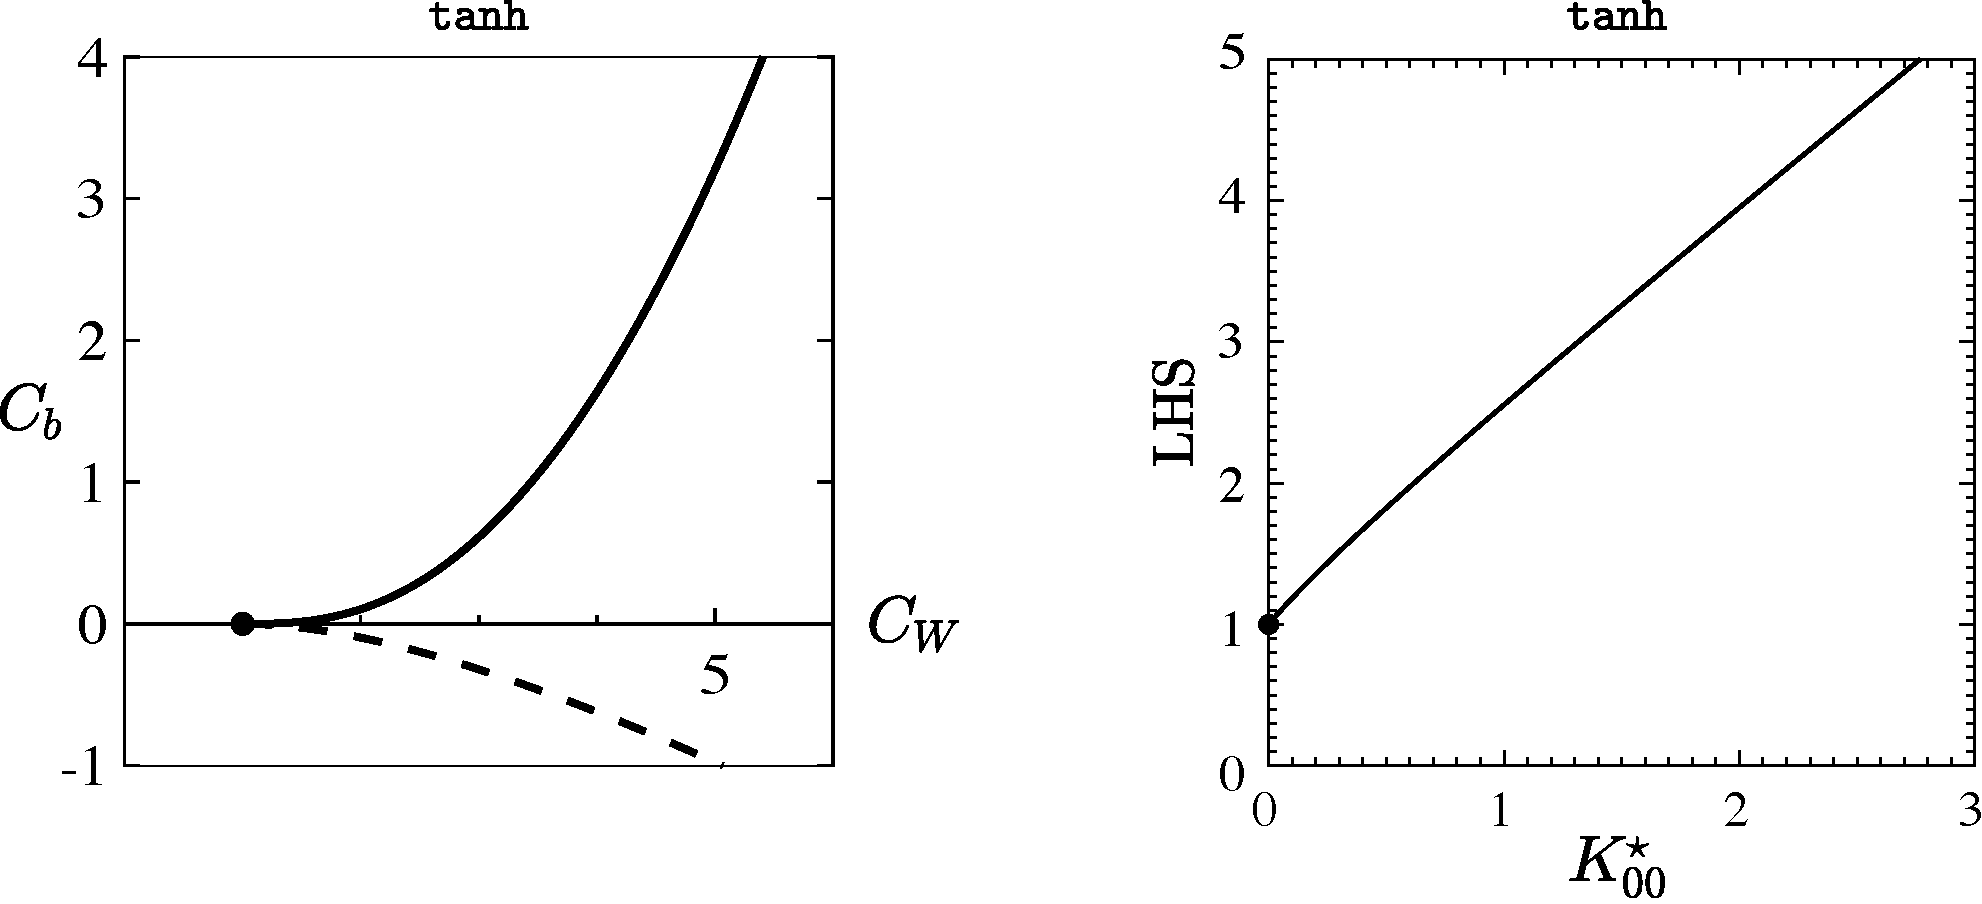
\includegraphics[width=0.85\linewidth]{./book_figures/algorithm_and_criticality_condition_tanh}
\end{center}
\caption{Two algorithms to pin down a nontrivial fixed point\index{fixed point!nontrivial}, illustrated here for the $\tanhA$ activation function. \textbf{Left:} the lines defined by the conditions $\Tif{\chi}{\perp}=1$ (solid) and $\Tif{\chi}{\parallel}=1$ (dashed) are shown in the hyperparameter plane $(C_W,C_b)$ for the $\tanhA$ activation function.
The intersection of these two lines gives the critical initialization hyperparameters $(C_W,C_b)=(1,0)$.
\textbf{Right:} the left-hand side of the condition~\eqref{easycriticality} is plotted as a function of $\Tif{\ker}{\M\M}$. The plotted line hits unity as $\Tif{\ker}{\M\M}\rightarrow 0$.
\index{initialization hyperparameters!critical}
}
\label{fig:tanh_critical}
\end{figure}



This algorithm, however, is practically cumbersome to carry out for general activation functions, both numerically and analytically. In order to obtain a more implementation-friendly algorithm, let's reshuffle the logic a bit.
First, note that for a candidate fixed-point value $\Tif{\ker}{\M\M}$, setting
\begin{align}
\label{CWcri}
C_W&=\le[ \bra\sigma'(z)\sigma'(z) \ket_{\Tif{\ker}{\M\M}}\ri]^{-1} \, ,\\ %
\label{Cbcri}
C_b&=\Tif{\ker}{\M\M}-\frac{\bra\sigma(z)\sigma(z) \ket_{\Tif{\ker}{\M\M}}}{\bra\sigma'(z)\sigma'(z) \ket_{\Tif{\ker}{\M\M}}} \, ,
\end{align}
satisfies both the fixed-point equation $\Tif{\ker}{\M\M}=C_b+C_W g_0\!\le(\Tif{\ker}{\M\M}\ri)$ as well as the first \terminate{criticality} condition $\chi_{\perp}\!\le(\Tif{\ker}{\M\M}\ri)=1$.
The second \terminate{criticality} condition $\chi_{\parallel}\!\le(\Tif{\ker}{\M\M}\ri)=1$ then is tantamount to $\chi_{\perp}\!\le(\Tif{\ker}{\M\M}\ri)/\chi_{\parallel}\!\le(\Tif{\ker}{\M\M}\ri)=1$, which is simply the following ratio of expectations
\be\label{easycriticality}
\le[\frac{2\ker^2 \bra\sigma'(z)\sigma'(z)\ket_{\ker}}{\bra \sigma(z)\sigma(z)\le(z^2-K\ri)\ket_{\ker}}\ri]\Bigg\vert_{\ker=\Tif{\ker}{\M\M}}=1\, ,
\ee
independent of the \terminate{initialization hyperparameters} $C_W$ and $C_b$.
Therefore, we can use the following simpler algorithm:
\begin{enumerate}
\item Scan over values of $\Tif{\ker}{\M\M}\geq 0$ until \eqref{easycriticality} is satisfied.
\item Plug the resulting value of $\Tif{\ker}{\M\M}$ into~\eqref{CWcri} and~\eqref{Cbcri} to evaluate the critical initialization hyperparameters (and also make sure $C_b\geq0$).
\end{enumerate}
In Figure \ref{fig:tanh_critical}, the left-hand side of~\eqref{easycriticality} is plotted as a function of $\Tif{\ker}{\M\M}$ for the $\tanhA$ activation function, which we see hits unity at $\Tif{\ker}{\M\M}=0$. \index{initialization hyperparameters!critical} Then, evaluating equations~\eqref{CWcri} and~\eqref{Cbcri} in the limit $\Tif{\ker}{\M\M}\rightarrow0$ efficiently gives the critical initialization hyperparameters for $\tanhA$: $(C_W,C_b)=(1,0)$\index{universality class!K@$K^\star=0$}.\footnote{
Even though the fixed-point value of the midpoint kernel\index{kernel!midpoint} is zero, this is a \emph{nontrivial} fixed point.\index{fixed point!nontrivial} In particular, we will see in~\S\ref{subsec:tanh_univ} that kernels with a nontrivial fixed point\index{fixed point!nontrivial} at $\Tif{\ker}{\M\M}=0$ form a \emph{universality class}, characterized by a benign power-law decay in $\ell$. In practice, the power-law behavior means that for any finite depth the kernel will remain finite.}
\index{universality class!K@$K^\star=0$}


\index{initialization hyperparameters!critical!for scale-invariant universality}\index{universality class!scale-invariant}
In passing, we note that scale-invariant activation functions trivially satisfy the condition~\eqref{easycriticality} for any fixed-point value $\Tif{\ker}{\M\M}$, since the susceptibilities are equal to the same kernel-independent constant, $\chi_{\parallel}\!\le(\ker\ri)=\chi_{\perp}\!\le(\ker\ri)=\chi$. It's easy to check that for this universality class, the above algorithm recovers the critical initialization hyperparameters~\eqref{eq:criticality_scale_invariant} given in~\S\ref{sec:scale-invariant-eft}.




\subsection{No Criticality: sigmoid, softplus, nonlinear monomials, etc.}\label{subsec:no_thinking_no_money}
For some activation functions, a nontrivial fixed point\index{fixed point!nontrivial} for the kernel does not exist. For example, consider the $\sigmoid$ activation function
\be
\sigma(z)=\frac{1}{1+e^{-z}}\, .
\ee
The condition~\eqref{easycriticality} is plotted for this activation in Figure~\ref{fig:no-crit}. While this condition is satisfied at  $\Tif{\ker}{\M\M}=0$, evaluating \eqref{Cbcri} in this limit yields $C_b=-\le(\frac{\sigma(0)}{\sigma'(0)}\ri)^2<0$. Since the variance of the bias cannot be negative, this is unphysical.\footnote{The limiting value of $C_b=-\le(\frac{\sigma(0)}{\sigma'(0)}\ri)^2$ hints that the conditions $\sigma(0)=0$ and $\sigma'(0) \neq 0$ may be necessary constraints for an activation function to have a nontrivial fixed point.}
Thus, the $\sigmoid$ cannot be tuned to \terminate{criticality} and should not be used.\footnote{Similarly, as a non-smooth limit of a \terminate{logistic function}, the $\perc$ activation function is even worse and doesn't merit discussion.}
\begin{figure}[h]
\begin{center}
 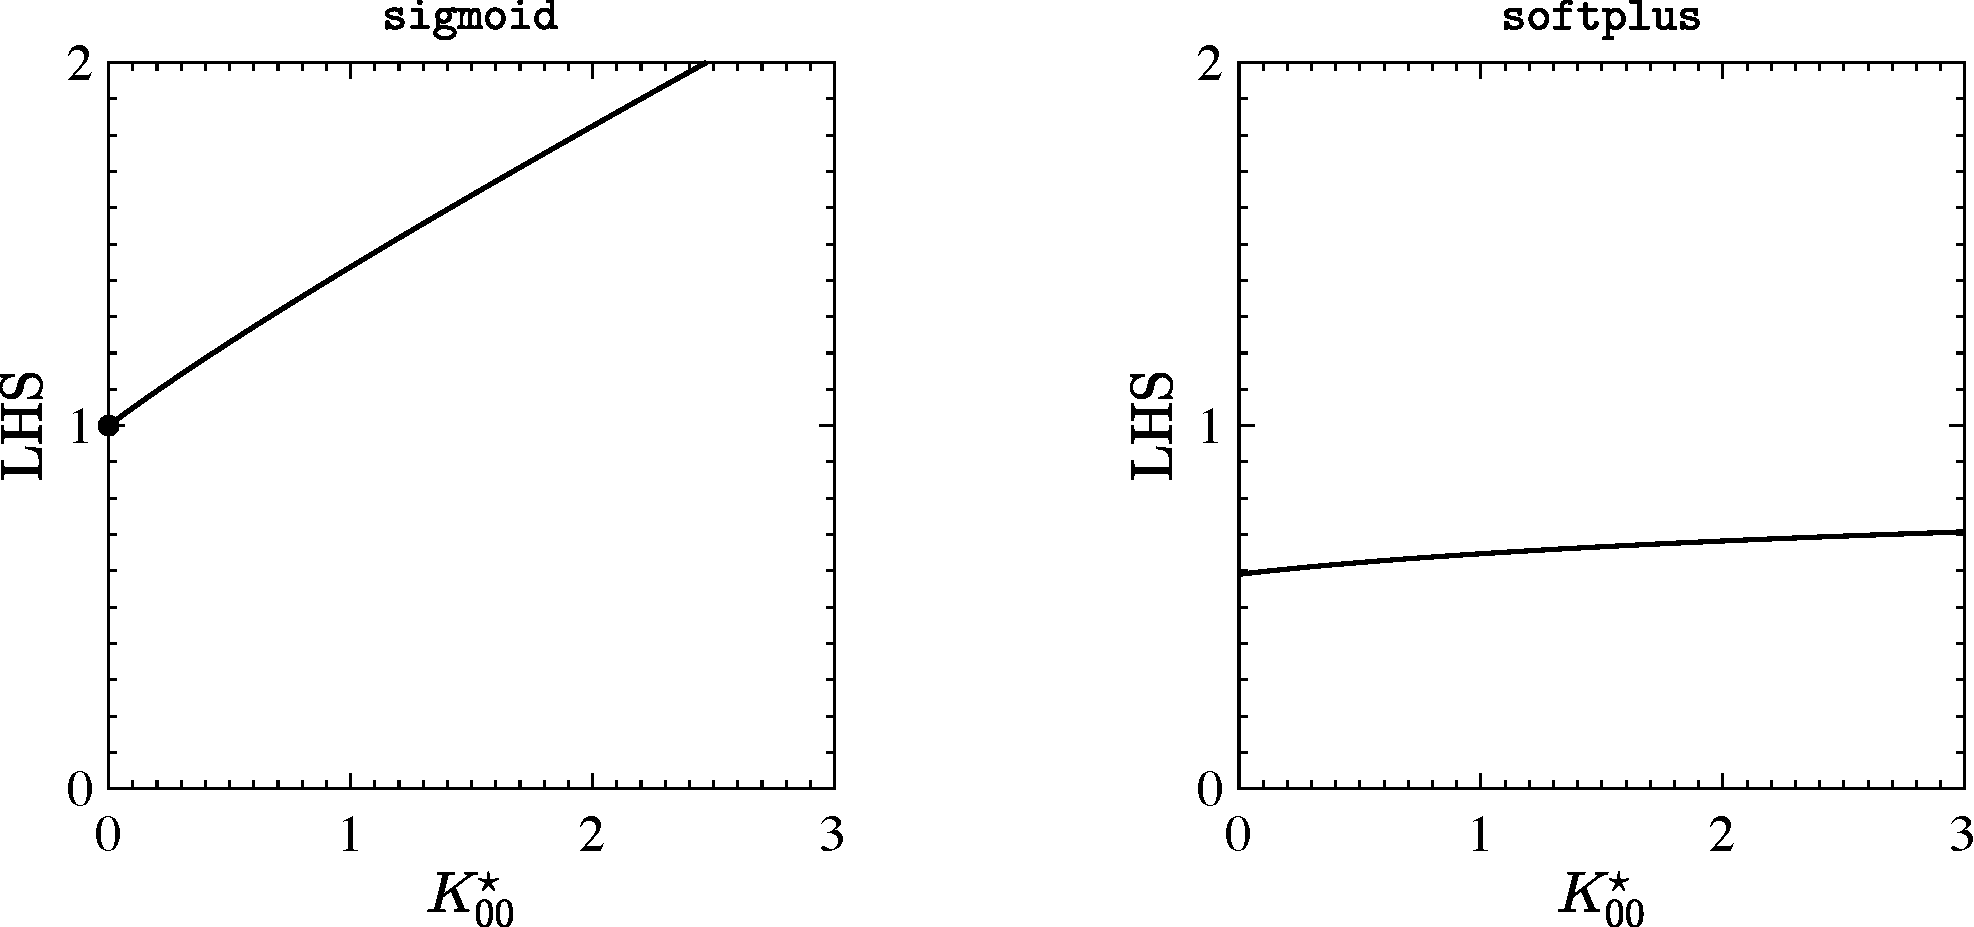
\includegraphics[width=0.85\linewidth]{./book_figures/criticality_sigmoid_and_softplus}
\end{center}
\caption{The left-hand side of the condition~\eqref{easycriticality} is plotted as a function of $\Tif{\ker}{\M\M}$ for the $\sigmoid$ activation function (left) and the $\softplus$ activation function (right).
For the $\sigmoid$, the plotted line hits unity as $\Tif{\ker}{\M\M}\rightarrow 0$, but the associated critical initialization hyperparameters $(C_b,C_W)$ are unphysical because $C_b<0$.
For the $\softplus$, the plotted line does not hit unity.
These activation functions cannot be tuned to \terminate{criticality}.}
\label{fig:no-crit}
\end{figure}


Next let's consider the $\softplus$ activation function
\be
\sigma(z)=\log\!\le(1+e^{z}\ri)\, ,
\ee
which, as a reminder, is a smooth approximation of the $\relu$.
Plotting the condition~\eqref{easycriticality} in Figure~\ref{fig:no-crit}, we see that it cannot be satisfied for any $\Tif{\ker}{\M\M}\geq0$.
Thus, in contrast to the $\relu$, the $\softplus$ cannot be tuned to \terminate{criticality}. This supports the lore in the community that the $\relu$ is superior to the $\softplus$, despite their similarity and the $\softplus$' smoothness.



As we will see in the next subsection, the real problem with these activation functions is that they do not cross zero at $z=0$. There is an easy fix, namely, setting
\be
\sigma(0)=0\, ,
\ee
by an appropriate constant shift for each activation. With such a shift the $\sigmoid$ turns into the $\tanhA$, albeit with the preactivation and activation each scaled by a half. Such a scaled $\tanhA$ indeed admits a critical initialization, which is easy to check after reading the discussion in the next subsection.


With that in mind, let's see what happens for activation functions that cross zero nonlinearly.
For simplicity, take any nonlinear $\texttt{monomial}$ activation function \index{activation function!monomial@\texttt{monomial}} 
\be
\sigma(z)=z^p\, ,  \quad p=2,3,4,\ldots\, .
\ee
In this case, direct Gaussian integration translates the condition~\eqref{easycriticality}  into the constraint
\be
\frac{p}{2p-1}=1 \, ,
\ee
which cannot be satisfied for nonlinear monomials, since $p\ne 1$. Thus, such nonlinear monomials also shouldn't be used in deep networks.
More importantly, in addition to $\sigma(0)=0$, \terminate{criticality} seems to require
the condition
\be
\sigma'(0)\ne 0\, ,
\ee
which we will investigate more generally in the next subsection.

The impossibility of \terminate{criticality} for all of the activation functions discussed in this subsection means that their use should be discouraged. While the problem is somewhat mitigated for shallow networks -- since there are fewer layers for the exponential behavior to damage the signals -- as networks become deeper and deeper, \terminate{criticality} becomes more and more essential.











\subsection{\texorpdfstring{$\Tif{\ker}{}=0$}{K*=0} Universality Class: tanh, sin, etc.}\label{subsec:tanh_univ}
\index{universality class!K@$K^\star=0$}

In \S\ref{subsec:strategize},  we learned through a numerical investigation that $\tanhA$ has a nontrivial fixed point\index{fixed point!nontrivial} at $\Tif{\ker}{\M\M}=0$. In addition, in the last subsection~\S\ref{subsec:no_thinking_no_money}, 
our analysis suggested
that the conditions $\sigma(0)=0$ and $\sigma'(0)\ne 0$ are %
important %
for any smooth activation to have a nontrivial fixed point\index{fixed point!nontrivial}. 

 \index{universality class!K@$K^\star=0$}
In this subsection, we will connect these two observations.
In particular,  in the vicinity of $\Tif{\ker}{\M\M}=0$, we can analytically analyze the kernel recursions \eqref{K0}--\eqref{K2} by Taylor expanding around $\Tif{\ker}{\M\M}=0$ and directly integrating the Gaussian expectations. This analysis will show that the conditions $\sigma(0)=0$ and $\sigma'(0)\ne 0$ are both necessary and sufficient for a smooth activation function to have a nontrivial fixed point at $\Tif{\ker}{\M\M}=0$, leading to the definition of our second universality class.



Let's use the following notation for the Taylor coefficients of any analytic activation function:
\be \label{eq:taylor-expansion-activation}
\sigma(z)=\sum_{p=0}^{\infty}\frac{\sigma_{p}}{p!}z^p\, .
\ee
Plugging this expansion into the definition of the helper function \eqref{eq:helper-function-general-strategy}  and performing the Gaussian integral, we find 
\be
g\!\le(\ker\ri)=\bra\sigma(z)\sigma(z) \ket_{\ker}=\sigma_0^2+\le(\sigma_1^2+2\sigma_0\sigma_2\ri)\ker+\o{\ker^2}\, .
\ee
From this we see that the fixed point of the recursion for the midpoint kernel\index{kernel!midpoint}
\be
\Tif{\ker}{\M\M}=C_b+C_W g\!\le(\Tif{\ker}{\M\M}\ri)\, ,
\ee 
has a solution at $\Tif{\ker}{\M\M}=0$  if and only if $C_b=C_W\sigma_0^2=0$.
Recalling that $C_W=0$ violates the \terminate{criticality} conditions, we must pick $\sigma_0=0$. Henceforth we will assume that this choice has been made.

Continuing on with $\sigma_0=0$ and $C_b =0$ in mind, inserting the expansion \eqref{eq:taylor-expansion-activation} into our expressions for the susceptibilities, \eqref{eq:chi-parallel} and \eqref{eq:chi-perp}, and performing the Gaussian integrals we find %
\begin{align}\label{eq:g0}
C_W g(\ker)
&=\le(C_W \sigma_1^2\ri)\le[K+a_1 K^2+a_2 K^3+\o{K^4}\ri]\, , \\
\label{eq:chi-parallel-expansion-K-star-equals-zero}
\chi_{\parallel}(\ker)%
&=\le(C_W \sigma_1^2\ri)\le[1+2 a_1K+3 a_2 K^2+\o{K^3}\ri]\, ,\\
\label{eq:chi-perp-expansion-K-star-equals-zero}
\chi_{\perp}(\ker)%
&=\le(C_W\sigma_1^2\ri)\le[1+b_1 K+\o{K^2}\ri]\, ,
\end{align}
where here we have also expanded $g(K)$ to higher order in the kernel, and the coefficients $a_1$, $a_2$, and $b_1$ are given by the following combinations of Taylor coefficients of the activation function
\begin{align}
\label{eq:a1}
a_1&\equiv \le(\frac{\sigma_3}{\sigma_1}\ri)+\frac{3}{4}\le(\frac{\sigma_2}{\sigma_1}\ri)^2\ ,\\
a_2&\equiv \frac{1}{4}\le(\frac{\sigma_5}{\sigma_1}\ri)+\frac{5}{8}\le(\frac{\sigma_4}{\sigma_1}\ri)\le(\frac{\sigma_2}{\sigma_1}\ri)+\frac{5}{12}\le(\frac{\sigma_3}{\sigma_1}\ri)^2\, ,\\
\label{eq:b1}
b_1&\equiv \le(\frac{\sigma_3}{\sigma_1}\ri)+\le(\frac{\sigma_2}{\sigma_1}\ri)^2\, .%
\end{align}
It's easy to check that, e.g., for $\tanhA$ these coefficients take the following values
$a_1=-2$, $a_2=17/3$, $b_1=-2$.
Now, examining expansions \eqref{eq:chi-parallel-expansion-K-star-equals-zero} and \eqref{eq:chi-perp-expansion-K-star-equals-zero}, we see that to satisfy the \terminate{criticality} conditions $\chi_{\parallel}\!\le(\Tif{\ker}{\M\M}=0\ri)=1$ and $\chi_{\perp}\!\le(\Tif{\ker}{\M\M}=0\ri)=1$ we must set $C_W= 1/\sigma_1^2$. To ensure a finite variance, we also see that the activation function must have $\sigma_1\ne 0$.

Thus, for any smooth activation function to have a nontrivial fixed point\index{fixed point!nontrivial} at $\Tif{\ker}{\M\M}=0$, it is necessary and sufficient that $\sigma(z)$ satisfy
\be\label{eq:tanh_cri_condition}
\sigma_0=0\, , \qquad  \sigma_1\ne0\, .
\ee
For such an activation, the critical initialization hyperparameters are then given by \index{initialization hyperparameters!critical!for K@for $K^\star=0$ universality}
\be\label{eq:k-star-equals-zero-critical-initialization}
\le(C_b, C_W\ri)^{\text{critical}}=\le(0, \frac{1}{\sigma_1^2}\ri)\, .
\ee
Just to emphasize this a bit, any activation with these conditions \eqref{eq:tanh_cri_condition} initialized with \eqref{eq:k-star-equals-zero-critical-initialization} will have a nontrivial fixed point at $\Tif{\ker}{\M\M}=0$. The set of activation functions that vanish at the origin with a nonzero first derivative make up the
\textbf{\boldmath$K^\star=0$ universality class}.\index{universality class!K@$K^\star=0$|textbf}
The canonical class member is the $\tanhA$ activation function, though there are obviously a very large number of members in this class, e.g.~the $\sinA$ activation function is a member too. 



\index{initialization hyperparameters!critical}
Having determined the critical initialization hyperparameters, let's now try to understand the behavior of the kernel 
for the $K^\star=0$ universality class.
We will see that when tuned to \terminate{criticality} the activations satisfying \eqref{eq:tanh_cri_condition} all behave similarly under RG flow, with the large-depth behavior of the kernel depending only on the first few Taylor coefficients of $\sigma(z)$.
\index{representation group flow}















\subsubsection{Deep asymptotic analysis for the midpoint kernel}


Recalling the expansion  $\Ti{ \ker}{\M\M}{\ell}=\Tif{\ker}{\M\M}+\Delta\Ti{ \ker}{\M\M}{\ell}$ around the fixed point and considering the expansion \eqref{eq:g0} for $g(K)$, the  midpoint kernel\index{kernel!midpoint} recursion at $\Tif{ \ker}{\M\M}=0$ \terminate{criticality} becomes
\be\label{eq:K-star-equals-zero-single-input-imprecise}
\Ti{\Delta \ker}{\M\M}{\ell+1}=\Ti{ \Delta\ker}{\M\M}{\ell}+a_1\le(\Ti{ \Delta\ker}{\M\M}{\ell}\ri)^2+a_2\le(\Ti{\Delta \ker}{\M\M}{\ell}\ri)^3+O\!\le(\le(\Ti{ \Delta\ker}{\M\M}{\ell}\ri)^4\ri)\, .
\ee
Since the whole point of \terminate{criticality} is to alleviate exponential behavior, we expect a gentler decay back to the $\Ti{ \ker}{\M\M}{\ell}=0$ fixed point. 
With that in mind, let's plug a power-law ansatz $\Ti{\Delta\ker}{\M\M}{\ell}\sim\le(\frac{1}{\ell}\ri)^{p_\M}$ into \eqref{eq:K-star-equals-zero-single-input-imprecise}. Noting that $\le(\frac{1}{\ell+1}\ri)^{p_\M}=\frac{1}{\ell^{p_\M}}\le[1-\frac{p_\M}{\ell}+O\!\le(\frac{1}{\ell^2}\ri)\ri]$ and matching the leading terms on both sides, we get a solution 
\be\label{eq:initial-tanh-wthout-subleading}
\Ti{\Delta\ker}{\M\M}{\ell}=\le[\frac{1}{(-a_1)}\ri]\frac{1}{\ell}+ \ldots \, .%
\ee
Thus, the behavior at \terminate{criticality} is a mild power law decay, with a \term{critical exponent} $p_\M=1$. Such an exponent is said to be \emph{universal} for the $K^\star=0$ universality class, since it is completely independent of the details of the particular activation function.

Importantly, for this asymptotic solution to be consistent, we must have $(-a_1)>0$ to ensure the positivity of the kernel. If instead we had $(-a_1) <0$, then the asymptotic solution~\eqref{eq:initial-tanh-wthout-subleading} would be negative, making it invalid. In this case the fixed point would be unstable, exponentially repelling the kernel away from $\Tif{ \ker}{\M\M}=0$\index{universality class!scale-invariant}.\footnote{Generically, $(-a_1)<0$ implies that $\chi_{\parallel}>1$ away from $\Tif{ \ker}{\M\M}=0$,
which repels the midpoint kernel\index{kernel!midpoint} first with a power law and then exponentially. However, the semi-criticality\index{criticality!semi-criticality} that we discussed in \S\ref{sec:scale-invariant-eft} for scale-invariant activations was exceptional. For this universality class, $a_1=0$ and hence growth towards the fixed point at infinity is governed by a power law.} 
We will see in the next subsection that 
$\swish$ and $\gelu$ activation functions exhibit such an instability near $\Tif{ \ker}{\M\M}=0$.

Moreover, in the last subsection we suggested that an activation function that doesn't satisfy $\sigma(0)=0$ could be potentially salvaged with a constant shift. In particular, perhaps the $\softplus$ could be saved by subtracting a constant $\log(2)$ so that $\sigma(0)=0$? %
However, in this case we'd have $(-a_1)<0$, and the kernel will get repelled from the only candidate nontrivial fixed point at $\Tif{ \ker}{\M\M}=0$.
And since $\chi_{\parallel}(K)>1$ away from $K=0$, the midpoint kernel\index{kernel!midpoint} will diverge exponentially.
Thus, despite this attempt, we see that the $\softplus$ cannot be saved.



Returning to our solution~\eqref{eq:initial-tanh-wthout-subleading}, we can actually do quite a bit better than ``$\ldots$'' for the subleading asymptotic analysis. As a first guess to improve our ansatz, let's include a subleading $1/\ell^2$ term in $\Ti{\Delta\ker}{\M\M}{\ell}$. However, if we try to match terms on both sides of \eqref{eq:K-star-equals-zero-single-input-imprecise}, we'd find that there's no way of canceling the $1/\ell^3$ terms.
What we can do instead is to also add $\log(\ell) /\ell^2$ with an independent coefficient to our ansatz. This generates an additional $1/\ell^3$ term, allowing for a consistent solution.
Generally for any of the observables $\O^{(\ell)}$ that we will consider, the correct \term{scaling ansatz} for the large-$\ell$ asymptotic expansion  is of the form
\begin{align}\label{eq:master-scaling-ansatz}
\Ti{\O}{}{\ell} &= \le( \frac{1}{\ell} \ri)^{p_\O} \le[c_{0,0}+  c_{1,1} \le( \frac{\log \ell}{\ell} \ri) + c_{1,0}\le( \frac{ 1}{\ell}\ri) +  c_{2,2} \le(  \frac{\log^2 \ell}{\ell^2} \ri)+  \dots \ri]%
\notag \\
&= \le( \frac{1}{\ell} \ri)^{p_\O} \le[\sum_{s = 0}^\infty \sum_{q=0}^{s} c_{s,q} \le( \frac{\log^q \ell}{\ell^s}  \ri)\ri],
\end{align}
where the \terminate{critical exponent} $p_\O$ is expected to be universal for a given class, while the constants $c_{s,q}$ will depend on the details of a particular activation function.
Carrying this process forward for $\O^{(\ell)} = \Ti{\Delta\ker}{\M\M}{\ell}$, we can systematically determine the subleading behavior of the kernel perturbation as
\begin{align}\label{eq:tanh_asymptotic}
\Ti{\Delta\ker}{\M\M}{\ell}&=\le[\frac{1}{(-a_1)}\ri]\frac{1}{\ell}+\le[\frac{-(a_2-a_1^2)}{a_1^3}\ri]\frac{\log\!\le(\frac{\ell}{\ell_0}\ri)}{\ell^2}\, \\
&+\le[\frac{-\le(a_2-a_1^2\ri)^2}{a_1^5}\ri]\frac{\le[\log\!\le(\frac{\ell}{\ell_0}\ri)\ri]^2}{\ell^3}+\le[\frac{\le(a_2-a_1^2\ri)^2}{a_1^5}\ri]\frac{\log\!\le(\frac{\ell}{\ell_0}\ri)}{\ell^3}+O\!\le(\frac{1}{\ell^3}\ri)\, ,\nonumber
\end{align}
and with enough effort this asymptotic expansion can be refined to arbitrary degree by %
including the higher-order corrections according to the scaling ansatz \eqref{eq:master-scaling-ansatz} described above. 

Here, the constant $\ell_0$ is undetermined by this large-$\ell$ asymptotic analysis and nontrivially depends on the input norm through
\be
\Ti{\ker}{\M\M}{1}=\frac{1}{\sigma_1^2}\frac{1}{n_0}\sum_{i=1}^{n_0}\x{i}{0}^2\, ,
\ee
which sets the initial condition~\eqref{eq:kernel-initial-condition} for the kernel recursion~\eqref{eq:kernel-recursion-reminder} when the rescaled weight variance is set to \terminate{criticality}, $C_W=1/\sigma_1^2$.
To get a sense of what this means, let's assume that $\chi_{\parallel}(\ker)$ is monotonically decreasing for $\ker\geq0$ with $\chi_{\parallel}(0)=1$ -- as is true for $\tanhA$ --  and consider what happens when an input $\x{i}{0}$ has a very large magnitude. Such a large-norm input will lead to a large value for the first-layer midpoint kernel\index{kernel!midpoint}, $\Ti{\ker}{\M\M}{1} \gg 1$. 
In the range $0<k_{\sharp}<\Ti{\ker}{\M\M}{\ell}$, for some constant $k_{\sharp}$, the kernel $\Ti{\ker}{\M\M}{\ell}$ will decay quicker than $\chi_{\parallel}(k_{\sharp})^{\ell}$, with $\chi_\parallel(k_{\sharp})<1$, until it enters the power-law regime near $\Tif{\ker}{\M\M}=0$. The undetermined constant $\ell_0$ is
a remnant of this complicated crossover behavior, capturing the leading \neo{data dependence}\index{data dependence|seealso{data-dependent coupling}}\index{data dependence|seealso{connected correlator}} of the midpoint kernel. 

\index{representation group flow}
Additionally, the asymptotic expansion for the midpoint kernel\index{kernel!midpoint} \eqref{eq:tanh_asymptotic} has a nice interpretation under RG flow. While the critical exponent of the falloff $p_\M=1$ is generic for the universality class, we see that the coefficients of the terms do depend on the details of the activation function, albeit only the first few Taylor coefficients. In fact, for larger and larger $\ell$, the dependence is on fewer and fewer of the coefficients, with the leading term only depending on $a_1$, \eqref{eq:a1}. In this asymptotic limit, any activation function in the $K^\star=0$ universality class with the same first three Taylor coefficients around zero will be completely indistinguishable. Thus, from the representation group flow perspective, one of the results of having a deeper network is to make the particular details of the activation function %
more and more irrelevant.

\index{critical exponent}
Lastly, let us note for all aspiring ``activation designers'' out there that we can engineer critical exponents other than $p_\M = 1$ by fine-tuning the Taylor coefficients of the activation function. For example, if we set $a_1=0$ by balancing $\sigma_3$ and $\sigma_2$, then the kernel approaches a $\Tif{\ker}{\M\M}=0$ nontrivial fixed point\index{fixed point!nontrivial} with a $ 1/\sqrt{\ell}$ power law decay so long as $(-a_2)>0$.
The need for such tuning indicates that the $\sim 1/\ell$ behavior is generic for activation functions in the $K^\star=0$ universality class.\footnote{
    More precisely, we should have defined the $K^\star=0$ universality class with the requirement $a_1\neq0$. This in turn would lead us to define a whole family of universality classes labeled by the degree of fine tuning of the $a_1, a_2,$ etc., or equivalently labeled by the value of the critical exponent $p_\M$. %
}  %



\subsubsection{Deep asymptotic analysis for parallel perturbations}
Next, let's solve the $\Ti{\delta\ker}{[1]}{\ell}$ recursion for parallel perturbations. 
Plugging the expansion \eqref{eq:chi-parallel-expansion-K-star-equals-zero} for $\chi_\parallel(K)$ into the recursion \eqref{K1}, we get an algebraic equation
\be\label{eq:parallel-agebraic}
\Ti{\delta\ker}{[1]}{\ell+1}=\le[1+2a_1\Ti{ \Delta\ker}{\M\M}{\ell}+3a_2\le(\Ti{ \Delta\ker}{\M\M}{\ell}\ri)^2+O\!\le(\le(\Ti{ \Delta\ker}{\M\M}{\ell}\ri)^3\ri)\ri]\Ti{\delta \ker}{[1]}{\ell}\, .
\ee
Then, plugging in the large-$\ell$ solution for $\Ti{\Delta\ker}{\M\M}{\ell}$ \eqref{eq:tanh_asymptotic}
and a large-$\ell$ asymptotic expansion for $\delta \ker_{[1]}^{(\ell)}$ based on our \terminate{scaling ansatz}~\eqref{eq:master-scaling-ansatz}, we can solve
the resulting equation by matching the terms on both sides:
\be
\delta \ker_{[1]}^{(\ell)}= \frac{\delta_{\parallel}}{\ell^2}\le[1+\frac{2a_1\le(a_2-a_1^2\ri)}{a_1^3}\frac{\log\!\le(\frac{\ell}{\ell_0}\ri)}{\ell}+O\!\le(\frac{1}{\ell}\ri)\ri]\, .
\ee


\index{universality class!K@$K^\star=0$} Inspecting our solution, we identify our second \terminate{critical exponent} for the $K^\star=0$ universality class: $p_\parallel = 2$ corresponding to the $1/\ell^2$ falloff of $\delta \ker_{[1]}^{(\ell)}$. The particular value of this exponent is to be expected.
As noted before, the parallel perturbation is just a difference of single-input kernels for two inputs with differing norms, $\Ti{\ker}{[1]}{\ell}=\le(\Ti{\ker}{++}{\ell}-\Ti{\ker}{--}{\ell}\ri)/2$. The leading $1/\ell^2$ scaling occurs because the diagonal components $\Ti{\ker}{++}{\ell}$ and $\Ti{\ker}{--}{\ell}$ are governed by the same asymptotic behavior up to order $\log(\ell)/\ell^2$, including the same coefficients. Thus, the leading difference appears at order $1/\ell^2$, due to different input-dependent constants $\ell_+$ and $\ell_-$ in expansions analogous to \eqref{eq:tanh_asymptotic} for $\Ti{\ker}{++}{\ell}$ and $\Ti{\ker}{--}{\ell}$, with the undetermined constant $\delta_{\parallel}\propto \log\!\le(\ell_{+}/\ell_{-}\ri)$.
In this way, this constant explicitly carries the \terminate{data dependence} of the parallel perturbation.








\subsubsection{Deep asymptotic analysis for perpendicular perturbations}
Finally, let's conclude our analysis by solving the $\Ti{\delta \delta\ker}{[2]}{\ell}$ recursion for perpendicular perturbations. 
Let's begin by plugging the expansion \eqref{eq:chi-perp-expansion-K-star-equals-zero} for $\chi_\perp(K)$ into the recursion \eqref{K2}. Since we want to focus on perpendicular perturbations with $\sum_{i=1}^{n_0}  \x{i}{\M}\, \delta x_i = 0$, we will also turn off parallel perturbations by setting $\delta \ker_{[1]}^{(\ell)}=0$. Putting this all together gives an algebraic equation
\be
\Ti{\delta\delta \ker}{[2]}{\ell+1}=\le[1+b_1\Ti{ \Delta\ker}{\M\M}{\ell}+O\!\le(\le(\Ti{\Delta \ker}{\M\M}{\ell}\ri)^2\ri)\ri]\Ti{\delta\delta \ker}{[2]}{\ell}\, .
\ee
Plugging in the large-$\ell$ asymptotic solution for $\Ti{\Delta\ker}{\M\M}{\ell}$ and solving the resulting equation with another large-$\ell$  asymptotic expansion  for $\delta\delta \ker_{[2]}^{(\ell)}$ based on our \terminate{scaling ansatz} \eqref{eq:master-scaling-ansatz},
we get
\be\label{eq:perp-asymptotic-solution}
\delta\delta \ker_{[2]}^{(\ell)}= \frac{\delta^2}{\ell^{\frac{b_1}{a_1}}}\le[1+\frac{b_1\le(a_2-a_1^2\ri)}{a_1^3}\frac{\log\!\le(\frac{\ell}{\ell_0}\ri)}{\ell}+O\!\le(\frac{1}{\ell}\ri)\ri]\,  ,
\ee
where $\delta^2$ is another unfixed constant undetermined by the large-$\ell$ solution, in this case related nontrivially to the magnitude of the difference of the inputs: $\sum_{i=1}^{n_0}\le(\x{i}{+} -  \x{i}{-}\ri)^2$. Here we see that the presumptive \terminate{critical exponent}, $p_\perp \equiv b_1 / a_1$, depends mildly on the details of the activation function.

\index{universality class!K@$K^\star=0$}
However, note that something nice happens for odd activation functions such as $\tanhA$ and $\sinA$. In this case, we see from \eqref{eq:a1} and \eqref{eq:b1} that $a_1 = b_1$, giving us a bona fide critical exponent, $p_\perp = 1$, when restricting the universality class to odd activations. This means that perpendicular perturbations decay with the same power in $\ell$ as the midpoint kernel\index{kernel!midpoint} decays to the fixed point, $\sim 1/\ell$. Thus, at \terminate{criticality} the ratio $ \ker_{[2]}^{(\ell)} / \ker_{[0]}^{(\ell)}$ is fixed at the leading order, preserving the angles between nearby perpendicular inputs. Importantly, this ensures that the relationship between input points is conserved under the RG flow, even if the signals propagate through a very deep network.\index{representation group flow}

Furthermore, the milder falloff of the perpendicular perturbations suggests that they are in some sense more important than the parallel ones. 
This is because with enough depth the $\Ti{\ker}{[1]}{\ell}$ component will become subleading to the $\Ti{\ker}{[0]}{\ell}$ and the $\Ti{\ker}{[2]}{\ell}$ components, due to the $1/\ell^2$ scaling of the former compared to the $1/\ell$ scaling of the latter two.
For this reason, we are going to
ignore these parallel perturbations of the kernel going forward.


\subsection{Half-Stable Universality Classes: SWISH, etc.~and GELU, etc.}\label{subsec:half_stability}\index{fixed point!nontrivial!half-stable}\index{fixed point!nontrivial!half-stable|seealso{\texttt{SWISH}}}\index{fixed point!nontrivial!half-stable|seealso{\texttt{GELU}}}
In this final subsection, we consider two other semi-popular activation functions in order to explore nontrivial fixed points away from zero, $\ker_{\M\M}^{\star}\ne 0$.
 \begin{figure}[ht]
\begin{center}
 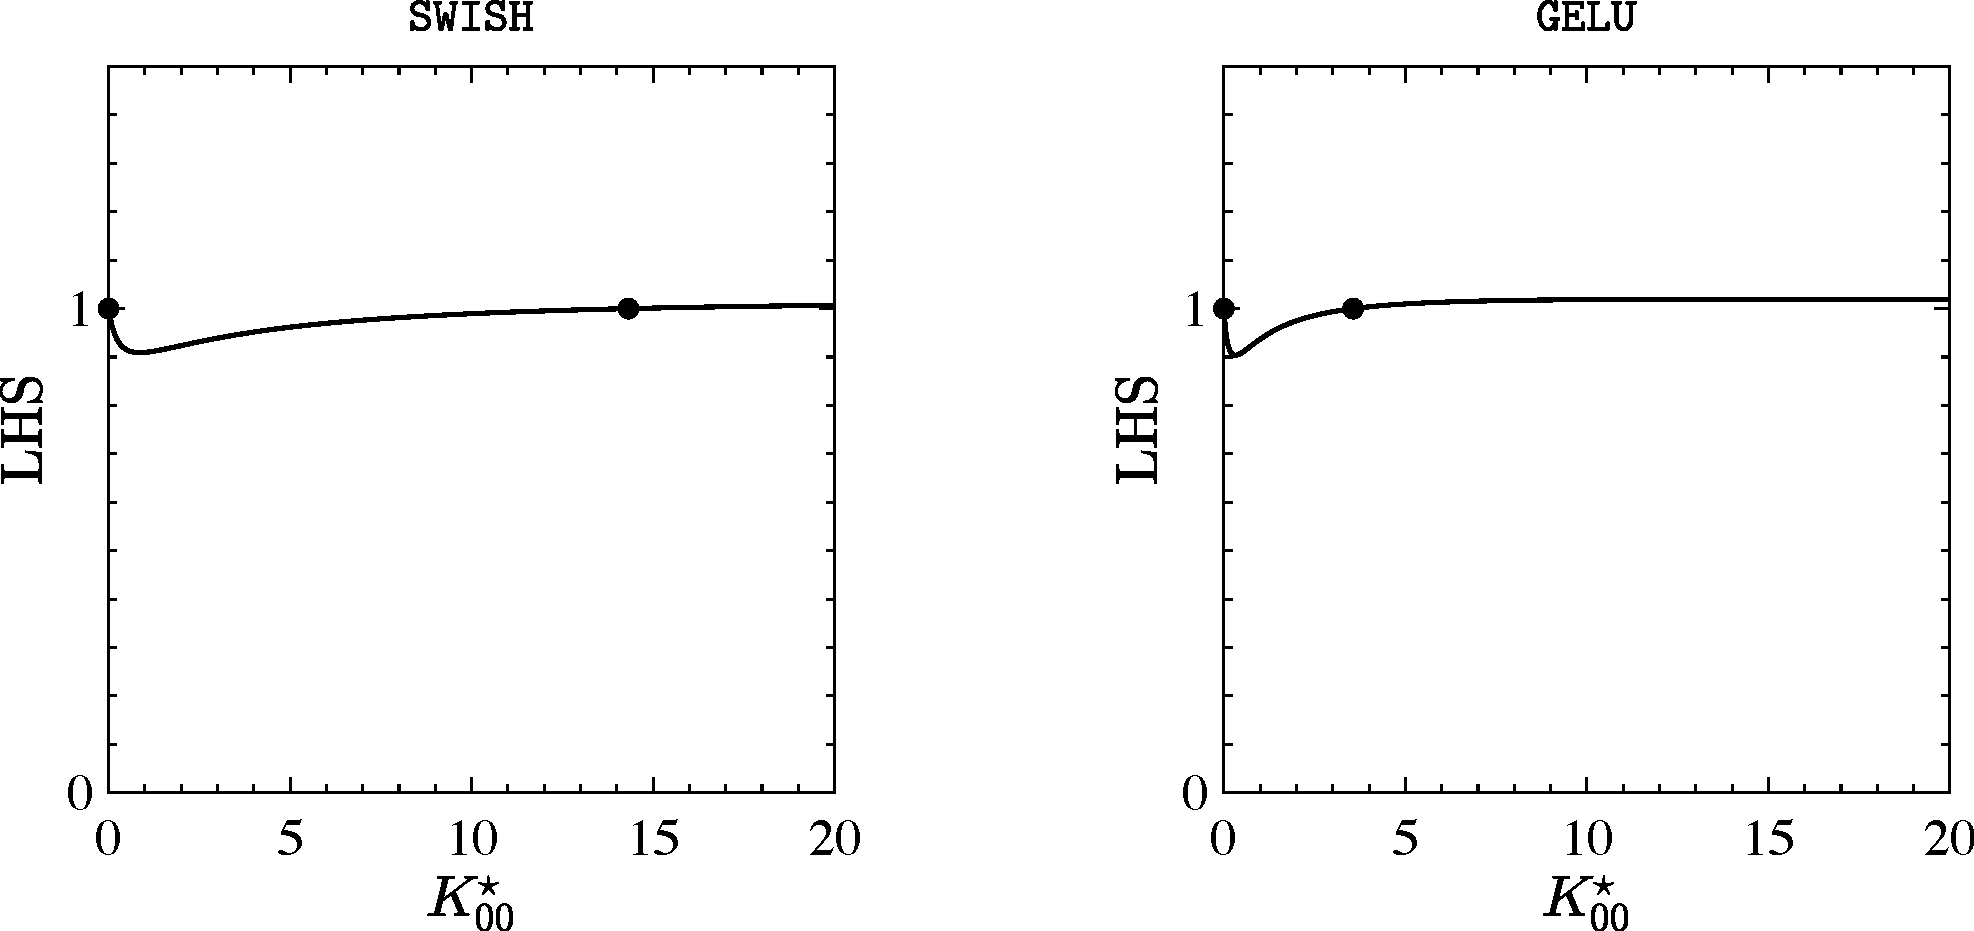
\includegraphics[width=0.85\linewidth]{./book_figures/criticality_condition_swish_and_gelu}
\end{center}
\caption{The left-hand side of the condition~\eqref{easycriticality} is plotted as a function of $\Tif{\ker}{\M\M}$ for the $\swish$ activation function (left) and the $\gelu$ activation function (right).
For both activation functions, the plotted line hits unity (black dots) at $\Tif{\ker}{\M\M}=0$ as well as at a nonzero half-stable nontrivial fixed point\index{fixed point!nontrivial!half-stable} $\Tif{\ker}{\M\M}\ne0$.}
\label{fig:half-crit}
\end{figure}
\begin{itemize}
\item The $\swish$ activation function is defined as
\be
\sigma(z)=\frac{z}{1+e^{-z}}\, .
\ee
Similar to the intuition for the $\softplus$, the $\swish$ is intended as a smooth version of the $\relu$.
Following our general algorithm in~\S\ref{subsec:strategize} for finding the critical initialization hyperparameters, we actually find two nontrivial fixed points for the kernel, see Figure~\ref{fig:half-crit}.  In particular, the condition~\eqref{easycriticality} is met at $\Tif{\ker}{\M\M}=0$ with $\le(C_b,C_W\ri)=\le(0,4\ri)$ and at
$\Tif{\ker}{\M\M}\approx 14.32017362$ with
\be\label{eq:swish-half-criticality}
\le(C_b,C_W\ri)\approx\le(0.55514317, 1.98800468\ri)\, .
\ee 
 For the $\Tif{\ker}{\M\M}=0$ nontrivial fixed point, one can check that $(-a_1)<0$, and hence it's unstable. For the $\Tif{\ker}{\M\M}\approx 14.3$ nontrivial fixed point, we expand the midpoint kernel\index{kernel!midpoint} recursion as $\KML=\Tif{\ker}{\M\M}+\Delta \KML$, yielding
 \be
\Delta \Ti{\ker}{\M\M}{\ell+1}=\Delta \Ti{\ker}{\M\M}{\ell}+\tilde{a}_1\le(\Delta \Ti{\ker}{\M\M}{\ell}\ri)^2+O\!\le(\le(\Delta \Ti{\ker}{\M\M}{\ell}\ri)^3\ri)\, ,
\ee
with 
$(-\tilde{a}_1)\approx-2.84979219\cdot 10^{-6}$. \index{initialization hyperparameters!critical} 

Here, the large-$\ell$ asymptotic analysis around the finite fixed point is identical to the case of $\Tif{\ker}{\M\M}=0$, resulting in
\be
\Delta \KML\sim\le[\frac{1}{\le(-\tilde{a}_1\ri)}\ri]\frac{1}{\ell} \, .
\ee
However, the interpretation is slightly different, because the fixed-point value $\Tif{\ker}{\M\M}\approx 14.3$ is non-vanishing. In particular, this implies that when $\KML<\Tif{\ker}{\M\M}$ the kernel is attracted to the fixed point, while when $\KML>\Tif{\ker}{\M\M}$ the kernel is repelled.\footnote{With the half-critical initialization hyperparameters for the $\swish$~\eqref{eq:swish-half-criticality}, there is a \emph{trivial} fixed point at $\Tif{\ker}{\M\M}\approx 14.5$ that exponentially attracts the midpoint kernel when $\KML>14.3$.} Hence, this fixed point is \textbf{half-stable}\index{fixed point!nontrivial!half-stable}, and so the activation function is perhaps half-useful. In practice, however,  $\vert \tilde{a}_1\vert $ is small enough that the $\swish$ behaves in an almost scale-invariant manner around $\KML\sim\Tif{\ker}{\M\M}\approx 14.3$.\index{scale invariance}
\index{fixed point!trivial}
 
\item The $\gelu$ activation is defined as 
\be
\sigma(z)=\frac{z}{2}\le[1+\text{erf}\le(\frac{z}{\sqrt{2}}\ri)\ri]\, ,
\ee
and as a reminder is another smoothed $\relu$.
Following our recipe for criticality, the condition~\eqref{easycriticality} is again met twice, at $\Tif{\ker}{\M\M}=0$ with $\le(C_b,C_W\ri)=\le(0,4\ri)$ and at
 $\Tif{\ker}{\M\M}=\frac{3+\sqrt{17}}{2}$ with
 \be\label{eq:gelu-half-criticality}
 \le(C_b,C_W\ri)\approx\le(0.17292239, 1.98305826\ri)\, ,
\ee
see Figure~\ref{fig:half-crit}.
Similar to the $\swish$, the fixed point at $\Tif{\ker}{\M\M}=0$ is unstable with $(-a_1)=-6/\pi<0$, and the fixed point at $\Tif{\ker}{\M\M}=\frac{3+\sqrt{17}}{2}$ is half-stable\index{fixed point!nontrivial!half-stable}, in this case with
$(-\tilde{a}_1)\approx (1.43626419)\cdot 10^{-4}$.
Note that the sign of $\tilde{a}_1$ here differs from the sign for the $\swish$.
Thus, this time, when $\KML>\Tif{\ker}{\M\M}$ the midpoint kernel is attracted to the fixed point, while when $\KML<\Tif{\ker}{\M\M}$ it is repelled.\footnote{With the half-critical initialization hyperparameters for the $\gelu$~\eqref{eq:gelu-half-criticality}, there is a \emph{trivial} fixed point at $\Tif{\ker}{\M\M}\approx 3.2$ that exponentially attracts the midpoint kernel when $\KML<\frac{3+\sqrt{17}}{2}\approx 3.6$.} \index{fixed point!trivial}
Note that the absolute value $\vert \tilde{a}_1\vert $ is bigger for the $\gelu$ than for the $\swish$, meaning that it behaves less scale-invariantly and looks less like the $\relu$. \index{scale invariance}
\end{itemize} \index{initialization hyperparameters!critical}\index{fixed point!nontrivial!half-stable}
Unlike the shifted $\softplus$ which admits only an unstable nontrivial fixed point at $\ker_{\M\M}^{\star}=0$, here the non-monotonicity of the $\gelu$ and $\swish$ activation functions gave rise to half-stable nontrivial fixed points at $\ker_{\M\M}^{\star}\ne 0$.
They are both representatives of \emph{half-stable universality classes}.\index{universality class!half-stable}
For both of these $\relu$-like activations functions, the critical initialization hyperparameters for the $\ker_{\M\M}^{\star}\ne 0$ half-stable nontrivial fixed points are very similar to the critical $\relu$ initialization $\le(C_b,C_W\ri) = (0,2)$;
the activations in each of these classes really are just small perturbations of the $\relu$. At the same time, the fact that there's a fixed point at a particular kernel value $\ker_{\M\M}^{\star}\ne 0$ indicates -- however weakly -- the introduction of a particular scale. This is one way to see that these universality classes break \terminate{scale invariance}.

In summary, despite being $\relu$-like and also smooth, both of the $\swish$ and $\gelu$ are inferior to the $\relu$ itself. If you want to use a smooth activation function, use $\tanhA$.









\section{Fluctuations}\label{sec:signal_prop_finite_width}



\index{$1/n$ expansion}\index{deep linear network}\index{representation group flow}
Now that we fully understand how to tune infinite-width networks
to \terminate{criticality}, let's back off this large-$n$ limit to analyze the behavior of realistic networks. Specifically, we're going to extend the finite-width analysis that we performed for deep linear networks in~\S\ref{sec:fluctuations_DLN} to MLPs with nonlinear activation functions.
Before diving in, let's review the motivation for carrying out such an analysis. %


\index{typicality}
First, note that practitioners only use a single network rather than an \terminate{ensemble} of networks.\footnote{Actually in some cases practitioners can use ensembles of networks, though the computational cost of such models grows in proportion to the number of networks in the ensemble.} 
As we have discussed, sometimes a single instantiation will generically deviate from the mean.
Therefore, in order to understand what \emph{typically} happens in a single instantiation for an observable of interest, we have to compute not only the mean but also instantiation-to-instantiation \terminate{fluctuations} around the mean. As we explained in \S\ref{sec:fluctuations_DLN}, such fluctuations are generically finite-width effects, controlled by the $1/n$-suppressed \terminate{four-point vertex} $\Ti{\FPV}{(\alpha_1\alpha_2)(\alpha_3\alpha_4)}{\ell}$.
If fluctuations are large, then a single instantiation can behave poorly, despite being sampled from an \terminate{initialization distribution} tune to \terminate{criticality}.


\index{statistical independence}\index{Gaussian distribution}\index{infinite-width limit}
Second, we saw in \S\ref{sec:deeper-layer-accumulation} that the infinite-width $\ell$-th-layer preactivation distribution factorizes as
\be\label{eq:infinite-distribution-factorization}
p\!\le(\zi{1}{\ell}, \dots, \zi{n_\ell}{\ell} \Big| \D \ri) = p\!\le(\zi{1}{\ell} \Big| \D \ri) \cdots p\!\le(\zi{n_\ell}{\ell} \Big| \D \ri) + \o{\frac{1}{n_\ell}} \, ,
\ee
where the distributions $p\!\le(\zi{i}{\ell} \Big| \D \ri)$ on each neuron are given by statistically independent Gaussian distributions.
(To emphasize the neural dependence here, we have included \terminate{neural indices} while suppressing \terminate{sample indices}.)
Recalling our discussion of \terminate{interactions} and statistical independence in \S\ref{sec:perturbation}, this means that intralayer correlations among neurons are entirely finite-width phenomenon.
Later, we will show how this lack of interactions connects to the fact that the representations\index{representation} of an infinite-width network cannot evolve during gradient-based learning. Thus, understanding these finite-width effects is a prerequisite to understanding how  
practical networks actually learn 
from input data\index{input data}.\footnote{We'll go into more detail about the role that these correlations play in the \terminate{inductive bias} of MLPs in~\S\ref{ch:bayesian-inference} and then connect these interactions to representation learning in~\S\ref{ch:features}.}




\index{metric!next-to-leading-order correction}\index{initialization hyperparameters!critical}\index{subleading corrections}
Third, finite-width corrections can modify the mean value of observables.
As we saw in~\S\ref{sec:loop-correction}, at finite width all observables in principle receive an infinite series of subleading corrections. For instance, a possible finite-width NLO correction to the metric, $\se{\alpha_1\alpha_2}{\ell}$, can shift the infinite-width metric, $G_{\alpha_1\alpha_2}^{\le\{0\ri\}(\ell)} \equiv \Ti{\ker}{\alpha_1\alpha_2}{\ell}$, a.k.a.~the \terminate{kernel}. 
Such a finite-width correction could potentially
ruin \terminate{criticality}, since our derivation of the critical initialization hyperparameters depended explicitly on the infinite-width fixed-point value of the kernel.\footnote{
    In \S\ref{subsec:relu_univ_revisit} we will show that the NLO metric $\se{\alpha_1\alpha_2}{\ell}=0$ vanishes for the scale-invariant universality class, which is why we didn't discuss this type of correction for deep linear networks\index{deep linear network} in \S\ref{ch:deep-linear-eft}.\index{universality class!scale-invariant}
} %





\index{metric!next-to-leading-order correction}\index{representation group flow}
There will be two main takeaways from this section.
\bi
\item First, we will find that the leading finite-width fluctuations scale with the depth-to-width ratio of the network, $L/n$. We saw the importance of this \neo{emergent scale} for the $\linear$ activation function in~\S\ref{sec:fluctuations_DLN}; here, we see that it persists very generally for nonlinear activation functions.
In the language of \S\ref{sec:marginalization-group-flow}, this means that finite-width corrections are \emph{relevant}\index{relevant (RG flow)} under representation group flow and that deeper networks deviate more and more from the simple \terminate{infinite-width limit}. This emphasizes the importance of including such corrections when analyzing such networks and -- taking into account the fact that overly deep networks suffer from overwhelming fluctuations -- suggests
that our perturbative \terminate{effective theory} works best in the regime where practical networks also work best.

\index{subleading corrections}\index{metric!next-to-leading-order correction}
\item Second,
the NLO metric $\se{\alpha_1\alpha_2}{\ell}$ is subdominant to the kernel $\Ti{\ker}{\alpha_1\alpha_2}{\ell}$ as long as an appropriate $\o{1/n}$ correction is made to 
$C_W$. This means that the NLO metric vanishes in the interpolating limit -- $n,L\rightarrow\infty$, with $L/n$ fixed -- and thus can safely be neglected
 for most wide networks of reasonable depths.
\ei



\subsubsection{A single input, reloaded}
In order to illustrate the important qualitative effects of finite width, we will again specialize to just a single input. 
The reason for this choice can be best understood by progressing through another twofold list: 
\bi
\item[\emph{(i)}] Once the two initialization hyperparameters, $C_b$ and $C_W$, are tuned to criticality at leading order by the one- and two-input analysis of the kernel, the only additional tuning comes from the single-input analysis of the NLO metric\index{metric!next-to-leading-order correction} $\se{\alpha_1\alpha_2}{\ell}$. Therefore, the multi-input solutions for the vertex and NLO metric\index{metric!next-to-leading-order correction} do not add anything to the \terminate{criticality} analysis.
\item[\emph{(ii)}]
The most interesting part of the two-input vertex is a component that gives variance of the input-output Jacobian\index{Jacobian!input-output} of the network. (As we described in footnote~\ref{footnote:Jacobian}, the mean value of this Jacobian is captured by 
the $\Ti{\ker}{[2]}{\ell}$ component of the kernel.) However, the would-be analysis of this input-output variance will be subsumed by our analysis of the variance of the \terminate{neural tangent kernel} in~\S\ref{ch:NTKa}, which more directly gives the variance of gradients relevant for training.
\ei 



In the rest of this section we'll omit the $\alpha=0$ \terminate{sample indices}, since such notation is unnecessarily cumbersome when considering only a single input. We'll also simplify things further by picking all the hidden-layer widths to be equal
\be\label{eq:chapter-eft-hidden-layer-widths-equal}
n_1=n_2=\cdots=n_{L-1}\equiv n \, .
\ee 
In addition to being a sensible choice, this means notationally that we don't have to carry around factors of $n_{\ell} / n_{\ell-1}$ everywhere.
With these decisions in mind, the relevant recursions from~\S\ref{ch:ngp} become
\begin{align}\label{eq:finite-width-reprinted-kernel}
\Ti{\ker}{}{\ell+1}&=C_b+C_W g\!\le(\Ti{\ker}{}{\ell}\ri)\, ,\\
\label{eq:finite-width-reprinted-vertex}
\Ti{\FPV}{}{\ell+1}&=\chi^2_{\parallel}\!\le(\Ti{\ker}{}{\ell}\ri)\Ti{\FPV}{}{\ell}+C_W^2\le[\bra \sigma^4(z) \ket_{\Ti{\ker}{}{\ell}}-\bra \sigma^2(z) \ket_{\Ti{\ker}{}{\ell}}^2\ri]\, ,\\
\label{eq:finite-width-reprinted-self-energy}
\se{}{\ell+1}&=\chi_{\parallel}\!\le(\Ti{\ker}{}{\ell}\ri)\se{}{\ell}+\frac{1}{8}\, j\!\le(\Ti{\ker}{}{\ell}\ri)\frac{\Ti{\FPV}{}{\ell}}{\le(\Ti{\ker}{}{\ell}\ri)^2}\, ,
\end{align}
where the helper function $g(K)$ and the parallel susceptibility $\chi_{\parallel}(K)$ were defined in~\eqref{eq:helper_first} and~\eqref{eq:chi-parallel}, and we have defined another
helper function
\be\label{eq:g4}
j(K)\equiv C_W\le\langle \sigma(z)\, \sigma(z)\!\le[\le(\frac{z^2}{K}\ri)^2-6\le(\frac{z^2}{K}\ri)+3\ri]\ri\rangle_{K}\, .
\ee
These three recursions can be solved for each universality class by mirroring our bootstrap analysis of $\Ti{\ker}{00}{\ell}$, $\Ti{\delta \ker}{[1]}{\ell}$, $\Ti{\delta\delta\ker}{[2]}{\ell}$ in \S\ref{sec:scale-invariant-eft} and \S\ref{sec:non-scale-invariant-eft}.







\subsection{Fluctuations for the Scale-Invariant Universality Class}\label{subsec:relu_univ_revisit}
Recall from~\S\ref{sec:scale-invariant-eft} that the scale-invariant universality class contains any activation function of the form \index{universality class!scale-invariant}
\be\label{eq:scale-invariant-reprinted}
\sigma(z) = 
    \begin{cases}
    a_+ z \, , & z \ge 0\, , \\
     a_- z \, , & z < 0  \, ,
    \end{cases}
\ee
with the $\relu$ $(a_+=1, a_-=0)$ as the exemplar member to keep in mind. Also recall that for this class we evaluated the helper function as $g(K)=A_2 K$ and the parallel susceptibility as $\chi_{\parallel}=A_2 C_W\equiv\chi$, with the activation-dependent constant given by $A_2\equiv (a_+^2+a_-^2)/2$. The other terms in the new recursions \eqref{eq:finite-width-reprinted-vertex} and \eqref{eq:finite-width-reprinted-self-energy} can similarly be evaluated by computing Gaussian integrals on the half-line, yielding
\be\label{eq:acctivation-function-gaussian-cov}
C_W^2\le[\bra \sigma^4(z) \ket_{\ker}-\bra \sigma^2(z) \ket_{\ker}^2\ri]= C_W^2\le(3A_4-A_2^2\ri)\ker^2\, , \qquad
j(K)=0\, ,
\ee
with a new activation-dependent constant 
\be
A_4\equiv\frac{a_+^4+a_-^4}{2} \, ,
\ee
to pair with our other constant, $A_2$.
With these expressions, the three recursions can be simplified as
\begin{align}\label{eq:kernel-scale-invariant-after-sub}
\Ti{\ker}{}{\ell+1}&=C_b+\chi \Ti{\ker}{}{\ell}\, ,\\
\label{eq:vertex-scale-invariant-after-sub}
\Ti{\FPV}{}{\ell+1}&=\chi^2\le(\frac{3A_4}{A_2^2}-1\ri)\le(\Ti{\ker}{}{\ell}\ri)^2+ \chi^2\,\Ti{\FPV}{}{\ell}\, ,\\
\se{}{\ell+1}&=\chi\, \se{}{\ell}\, . \label{eq:self-energy-scale-invariant-after-sub}
\end{align}
As a reminder, we already solved the kernel recursion in \S\ref{sec:scale-invariant-eft}.

\index{metric!next-to-leading-order correction}
Things are now quite simple. \index{universality class!scale-invariant}
\bi
\item First, remember from \S\ref{sec:first-layer-gaussian} that the first layer preactivation distribution is always exactly Gaussian, implying that the first-layer two-point correlator
is simply given in terms of the first-layer kernel $\Ti{\ker}{}{1}$ to all orders in $n$
\be\label{eq:two-point-first-layer-reprinted}
\E{z^{(1)}_i z^{(1)}_j}=\delta_{ij} \ker^{(1)} \, .
\ee
This means that the first-layer NLO metric\index{metric!next-to-leading-order correction} must vanish $\se{}{1}=0$, and recursion \eqref{eq:self-energy-scale-invariant-after-sub} then tell us that the NLO metric will vanish in any subsequent layer. Thus, for activations in the scale-invariant universality class, we learn that the single-input metric does not get corrected at $\o{1/n}$. 
\item Second, let's focus on \terminate{criticality} by setting $C_b=0$ and $C_W = 1/A_2$. As discussed in \S\ref{sec:scale-invariant-eft}, this setting of hyperparameters fixes the kernel to be an input-dependent layer-independent constant 
\be
\Ti{\ker}{}{\ell}=\Tif{\ker}{}\equiv\frac{1}{A_2} \le(\frac{1}{n_0}\sum_{i=1}^{n_0}x_i^2\ri) \, .
\ee
In particular, this means that the \terminate{critical exponent} for the single-input kernel is given by $p_0=0$. Setting $\chi=1$ and substituting this expression into \eqref{eq:vertex-scale-invariant-after-sub}, we find a linearly growing  solution for the \terminate{four-point vertex}
\be\label{eq:scale-invariant-vertex-solution}
\Ti{\FPV}{}{\ell}=\le(\ell-1\ri)\le(\frac{3A_4}{A_2^2}-1\ri) \le(\Tif{\ker}{}\ri)^2 \, .
\ee
By inspection, we identify another \terminate{critical exponent} for the scale-invariant universality class: assuming $V^{(\ell)}\sim (1/\ell)^{p_V}$, then $p_V=-1$. This exponent encodes the linear growth of the vertex under RG flow.
\index{universality class!scale-invariant}
Of particular note, the coefficient in front of \eqref{eq:scale-invariant-vertex-solution} evaluates to $\le(\frac{3 A_4}{A_2^2} -1\ri)= 2$ for $\linear$ activations in contrast to =$5$ for $\relu$ activations. Apparently the fluctuations in $\relu$ networks are significantly stronger than in deep linear networks\index{deep linear network}. More generally, we conclude that the strength of such fluctuations is \emph{not} universal.  


\index{universality class!scale-invariant}
\item
Third, let's revisit semi-criticality\index{criticality!semi-criticality}  by setting $C_W = 1/A_2$, but setting the bias variance to an arbitrary positive constant, $C_b>0$. As we saw in~\S\ref{sec:scale-invariant-eft},   
in this case the kernel grows linearly towards a nontrivial fixed point\index{fixed point!nontrivial} at infinity, $\Ti{\ker}{}{\ell}\sim \ell$, i.e., $p_0=-1$. Plugging such a solution into the vertex recursion \eqref{eq:vertex-scale-invariant-after-sub}, we see that the four-point vertex grows cubicly $\Ti{\FPV}{}{\ell} \sim \ell^3$, i.e., $p_V=-3$.  However, the appropriate dimensionless quantity
-- normalizing the vertex by the square of the kernel --
still grows linearly in $\ell$, i.e., $p_V-2p_0=-1$.\footnote{
To elaborate a bit more, first please reread~footnote~\ref{foot:dimensional-analysis} in \S\ref{sec:perturbation} on \neo{dimensional analysis}. Now, if we give the preactivations a dimension $[z]=\zeta$, then we have for the kernel $[\ker]=\zeta^2$, while for the four-point vertex $[\FPV]=\zeta^4$. Thus, the ratio $V/K^2$ is dimensionless.
}
Thus, even for semi-criticality\index{criticality!semi-criticality} the universal $\ell/n$-scaling of the finite-width corrections is preserved.\index{universality class!scale-invariant}
\ei



\subsection{Fluctuations for the \texorpdfstring{$\Tif{\ker}{}=0$}{K*=0} Universality Class}\label{subsec:tanh_univ_revisit}
Let's now consider the $K^{\star}=0$ universality class. As a reminder, this class contains all smooth activation functions that satisfy $\sigma(0)=0$ and $\sigma'(0)\ne0$, %
with $\tanhA$ as the exemplar member to keep in mind. 
In \S\ref{subsec:tanh_univ}, we determined that activations in this class have a nontrivial fixed point\index{fixed point!nontrivial} at $\Tif{\ker}{}=0$ and found that the associated critical initialization hyperparameters are given by $C_b=0$ and $C_W=1/\sigma_1^2$.
For the rest of this subsection
we will focus on such networks at \terminate{criticality}. %
\index{universality class!K@$K^\star=0$}\index{initialization hyperparameters!critical}

Mirroring our approach in \S\ref{subsec:tanh_univ} to solve the kernel recursions, we can evaluate the Gaussian expectations in the vertex recursion~\eqref{eq:finite-width-reprinted-vertex} and the NLO-metric recursion~\eqref{eq:finite-width-reprinted-self-energy} by Taylor expanding the activation around $z=0$ and explicitly computing the Gaussian integrals. Keeping in mind the \terminate{criticality} condition $C_W=1/\sigma_1^2$, this gives the following expressions 
\begin{align}\label{eq:chi-parallel-agebriac}
\chi_{\parallel}(K)&=1+2a_1\ker+3a_2\ker^2+\o{\ker^3}\, ,\\
\label{eq:first-part-of-vertex-algebriac}
C_W^2\le[\bra \sigma^4(z) \ket_{\ker}-\bra \sigma^2(z) \ket_{\ker}^2\ri]&= 2 \ker^2+\le(-52a_1+60b_1\ri)K^3+\o{\ker^4}\, , \\
\label{eq:g4-algebriac-k-star}
\frac{j(K)}{8 \ker^2}&= a_1 +3 a_2 \ker+\o{\ker^2}\, .
\end{align}
Here, the expression for $\chi_{\parallel}\!\le(\ker\ri)$ is simply reprinted from~\S\ref{subsec:tanh_univ}. Similarly, to limit the amount of time you have to flip back and forth, let us also reprint the large-$\ell$ asymptotic expansion of the kernel perturbation originally given by~\eqref{eq:tanh_asymptotic}:
\begin{align}\label{k-star-equals-zero-kernel-solution-reprinted}
\Ti{\Delta \ker}{}{\ell}&=\le[\frac{1}{(-a_1)}\ri]\frac{1}{\ell}+\le[\frac{-(a_2-a_1^2)}{a_1^3}\ri]\frac{\log\!\le(\frac{\ell}{\ell_0}\ri)}{\ell^2}\, \\
&+\le[\frac{-\le(a_2-a_1^2\ri)^2}{a_1^5}\ri]\frac{\le[\log\!\le(\frac{\ell}{\ell_0}\ri)\ri]^2}{\ell^3}+\le[\frac{\le(a_2-a_1^2\ri)^2}{a_1^5}\ri]\frac{\log\!\le(\frac{\ell}{\ell_0}\ri)}{\ell^3}+\o{\frac{1}{\ell^3}}\, .\nonumber
\end{align}

\subsubsection{Four-Point Vertex}
Now, let's find a solution for the \terminate{four-point vertex}.
Substituting in \eqref{eq:chi-parallel-agebriac} and \eqref{eq:first-part-of-vertex-algebriac} into the single-input vertex recursion \eqref{eq:finite-width-reprinted-vertex} gives an algebraic equation
\begin{align}
\Ti{\FPV}{}{\ell+1}&=\Ti{\FPV}{}{\ell}\le[1+4a_1 \Ti{\Delta\ker}{}{\ell}+\le(6a_2+4a_1^2 \ri) \le(\Ti{\Delta\ker}{}{\ell}\ri)^2+\ldots\ri]\,  \\
&+2 \le(\Ti{\Delta\ker}{}{\ell}\ri)^2+\le(-52a_1+60b_1\ri) \le(\Ti{\Delta\ker}{}{\ell}\ri)^3+\ldots\, .\nonumber
\end{align}
Using our \terminate{scaling ansatz}~\eqref{eq:master-scaling-ansatz} for the large-$\ell$ asymptotic expansion
\be\label{eq:vertex-scaling-ansatz}
\Ti{\FPV}{}{\ell} =\le( \frac{1}{\ell} \ri)^{p_V} \le[\# +  \#' \frac{\log \ell}{\ell}  +   \frac{\#''}{\ell} +  \ldots \ri]\, ,
\ee
and \eqref{k-star-equals-zero-kernel-solution-reprinted} for $\Ti{\Delta \ker}{}{\ell}$ and then
matching terms, we find 
\begin{align}\label{eq:Kstar-equals-zero-vertex-solution}
\Ti{\FPV}{}{\ell}&=\le[\frac{2}{3a_1^2}\ri]\frac{1}{\ell}+\le[\frac{2(a_2-a_1^2)}{3 a_1^4}\ri]\frac{\log\!\le(\frac{\ell}{\ell_0}\ri)}{\ell^2}\, \\
&+\le[\frac{5a_2+a_1(82 a_1-90 b_1)}{3 a_1^4}\ri]\frac{1}{\ell^2}+\o{\frac{\log^2(\ell)}{\ell^3}}\, , \nonumber
\end{align}
where the constant scale $\ell_0$ is same as the one in the $\Ti{\Delta\ker}{}{\ell}$ expansion
just above, again carrying the \terminate{data dependence} of the solution.
We can also read off the \terminate{critical exponent} controlling the asymptotic falloff of the vertex for the $K^\star=0$ universality class:  
 $p_V=1$.%

\index{universality class!scale-invariant}\index{universality class!K@$K^\star=0$}
Note that the value of the exponent $p_V=1$ and the behavior of the four-point vertex $V^{(\ell)}\sim  1/\ell$ here is different from the value of the exponent $p_V=-1$ and the associated behavior $V^{(\ell)}\sim \ell$  that we found for the scale-invariant universality class. Also note that we saw this difference in the behavior of the kernel, $p_0=1$ vs.~$p_0=0$, for the $K^\star=0$ and scale-invariant classes, respectively. However, when instead considering the dimensionless quantity
\be\label{eq:k-star-equals-zero-normalized-four-point-scaling-law}
\frac{\Ti{\FPV}{}{\ell}}{n \le(\Ti{ \ker}{}{\ell} \ri)^2} \sim  \frac{1}{n}\le(\frac{1}{\ell} \ri)^{p_V-2p_0} + \dots \, ,%
\ee
we see that its scaling is consistent across both classes of activations:
\be\label{eq:vertex-scaling-law}
p_V-2p_0 = -1\, .
\ee
Thus, this \term{scaling law} holds across different universality classes. \index{universality class!transcended by scaling laws}
As the normalized quantity \eqref{eq:k-star-equals-zero-normalized-four-point-scaling-law} controls leading finite-width corrections to observables  -- this was discussed in detail in 
\S\ref{sec:fluctuations_DLN} --  such a law means that these corrections are always \emph{relevant}\index{relevant (RG flow)} under \terminate{representation group flow}.


Concretely, the normalized vertex function is given by 
\be\label{eq:k-star-equals-zero-normalized-four-point-relu-univ}
\frac{\Ti{\FPV}{}{\ell}}{n \le(\Ti{ \ker}{}{\ell} \ri)^2} = \le(\frac{3 A_4}{A_2^2} -1\ri)  \frac{\ell}{n} + \o{\frac{1}{n}} \, ,
\ee
for the scale-invariant universality class
and 
\be\label{eq:k-star-equals-zero-normalized-four-point-tanh-univ}
\frac{\Ti{\FPV}{}{\ell}}{n \le(\Ti{ \ker}{}{\ell} \ri)^2} = \le(\frac{2}{3}\ri)\frac{\ell}{n} + \o{\frac{\log \le(\ell\ri)}{n}} \, ,
\ee
for the $\ker^{\star}=0$ universality class. 
Of practical relevance, this means that $\relu$ networks and $\tanhA$ networks of the same depth and width will have a mostly similar sensitivity to such corrections. However, the $\o{1}$ coefficient of this quantity \emph{does} depend on the particular activation function: =$5$ for $\relu$ and =$2/3$ for $\tanhA$. In Appendix~\ref{app:mi-stuff}, we'll analyze this a bit more using tools from \neo{information theory} and see how it can lead to a preferred aspect ratio, $L/n$, that is different for specific choices of activation functions.
\index{universality class!scale-invariant}\index{universality class!K@$K^\star=0$}





\subsubsection{NLO metric, bare}
\index{metric!next-to-leading-order correction}\index{subleading corrections}\index{metric!next-to-leading-order correction}
Next, let's solve the NLO-metric recursion \eqref{eq:finite-width-reprinted-self-energy}. 
Substituting in \eqref{eq:chi-parallel-agebriac} for $\chi_{\parallel}(K)$ and \eqref{eq:g4-algebriac-k-star} for $j(K)$, we get
\be\label{eq:nlo-metric-recursion-bare}
\se{}{\ell+1}=\se{}{\ell}\le[1+2a_1 \Ti{\Delta\ker}{}{\ell}+\ldots\ri] +\Ti{\FPV}{}{\ell}\le[a_1+3a_2  \Ti{\Delta\ker}{}{\ell}+\ldots\ri]\, .
\ee
As should now be familiar, let's assume a large-$\ell$ \terminate{scaling ansatz}
\be\label{eq:nlo-metric-scaling-ansatz}
\se{}{\ell}= \# \le( \frac{1}{\ell} \ri)^{p_1}+ \ldots \, ,
\ee
with $p_1$ as the associated \terminate{critical exponent}.
Bootstrapping \eqref{eq:nlo-metric-recursion-bare} by substituting in our previous solutions -- \eqref{k-star-equals-zero-kernel-solution-reprinted} for $\Delta\ker^{(\ell)}$  and \eqref{eq:Kstar-equals-zero-vertex-solution} for $\Ti{\FPV}{}{\ell}$ -- we then insert our ansatz  for $\se{}{\ell}$ \eqref{eq:nlo-metric-scaling-ansatz} and match terms to find 
\be\label{eq:k-star-equal-zero-self-energy}
\se{}{\ell}= -\le[\frac{1}{3(-a_1)}\ri]+ \o{\frac{\log \le(\ell\ri)}{\ell}} \, .
\ee
This solution required us to set $p_1 = 0$ and gave a constant-in-$\ell$ leading contribution.
Combining this with the kernel, we see that the finite-width-corrected two-point correlator 
\be\label{eq:two-point-with-leading-finite-width-reprinted}
\E{z^{(\ell)}_i z^{(\ell)}_j}=\delta_{ij} \le[\ker^{(\ell)} + \frac{1}{n}\se{}{\ell}+\o{1/n^2}\ri] \, ,
\ee
is given by
\be\label{eq:k-star-full-two-point-with-self-energy}
\ker^{(\ell)} + \frac{1}{n}\se{}{\ell} = \le[\frac{1}{(-a_1)}\ri]\le(\frac{1}{\ell} -\frac{1}{3n}\ri)+ \ldots\, . %
\ee
This result is to be contrasted with the scale-invariant universality class, where the NLO metric\index{metric!next-to-leading-order correction} vanished identically. 

\index{critical exponent}\index{subleading corrections}\index{metric!next-to-leading-order correction}
For the NLO metric\index{metric!next-to-leading-order correction}, the appropriate dimensionless quantity to consider is the ratio between the correction term and the infinite-width term in the two-point correlator \eqref{eq:two-point-with-leading-finite-width-reprinted}
\be\label{eq:nlo-dimensionless-ratio}
\frac{1}{n}\frac{\se{}{\ell}}{\ker^{(\ell)}} \sim  \frac{1}{n}\le(\frac{1}{\ell}\ri)^{p_1-p_0}+ \dots \, ,
\ee
with the exponent $p_1 - p_0$ controlling the relative importance of this NLO correction. In this case we see that $p_1-p_0=-1$, meaning that the above ratio scales with the depth-to-width ratio $\ell/n$.
This again illustrates the perturbative cutoff\index{cutoff, effective theory} of our \terminate{effective theory}, $\ell \lesssim n$.
However, in this particular case such a scaling turns out to be an artifact of not properly tuning the initialization hyperparameters $C_W$ at finite width, as we will see next.
\index{universality class!scale-invariant}



\subsubsection{NLO metric, renormalized}
\index{renormalization group flow}\index{metric!next-to-leading-order correction}\index{$1/n$ expansion}\index{initialization hyperparameters!critical!at finite width}\index{universality class!K@$K^\star=0$}\index{subleading corrections}\index{metric!next-to-leading-order correction}


In \S\ref{subsec:tanh_univ}, we learned how to find the critical initialization hyperparameters for the $K^\star=0$ universality class, fixing the hyperparameters $C_b$ and $C_W$ using the infinite-width recursions for the kernel components. However, in \S\ref{sec:loop-correction} we explained that all of the observables computed in a large-$n$ expansion receive an infinite series of subleading corrections in $1/n$.  This suggests that we should have allowed further fine-tuning of the initialization hyperparameters at \terminate{criticality} by considering large-$n$ expansions
\begin{align}
\label{eq:Cb-expansion}
\Cb{\ell} &= \cbn{\ell}{0} + \frac{\cbn{\ell}{1}}{n_{\ell-1}} +\frac{\cbn{\ell}{2}}{n_{\ell-1}^2} + \dots \, , \\
\label{eq:CW-expansion}
\CW{\ell} &= \cWn{\ell}{0} + \frac{\cWn{\ell}{1}}{n_{\ell-1}} +\frac{\cWn{\ell}{2}}{n_{\ell-1}^2} + \dots \, ,
\end{align}
allowing us to adjust such hyperparameters order by order in $1/n$. Such an expansion could potentially give additional criticality conditions at each order in perturbation theory.

\index{subleading corrections}\index{metric!next-to-leading-order correction}
Considering the finite-width recursions \eqref{eq:finite-width-reprinted-vertex} and \eqref{eq:finite-width-reprinted-self-energy}, we see that such subleading tunings will not affect the leading order result for observables that depend on the \terminate{four-point vertex}, since the leading contributions to such observables are already at $\o{1/n}$. However, these tunings do affect the solution for the NLO metric\index{metric!next-to-leading-order correction}, because the NLO metric is itself subleading. 



Concretely, there is an additional contribution to the NLO-metric recursion \eqref{eq:finite-width-reprinted-self-energy} coming from inserting the expansions \eqref{eq:Cb-expansion} and \eqref{eq:CW-expansion} into the kernel recursion \eqref{eq:finite-width-reprinted-kernel}. The terms proportional to $\cbn{\ell}{1}$ or $\cWn{\ell}{1}$ are now subleading and thus contribute to the NLO metric\index{metric!next-to-leading-order correction} recursion: 
\be\label{eq:nlo-metric-recursion-renormalized}
\se{}{\ell+1}= \le[\cbn{\ell}{1} + \cWn{\ell}{1} g\!\le(K^{(\ell)}\ri) \ri]+ \chi_{\parallel}^{(\ell)}\se{}{\ell}+ \frac{1}{8}\, j\!\le(\Ti{\ker}{}{\ell}\ri) \frac{\Ti{\FPV}{}{\ell}}{\le(\Ti{\ker}{}{\ell}\ri)^2}   \, .
\ee 
With this new ``renormalized'' perspective, we see that the analysis we did in the ``bare'' subsubsection before was just a particular choice of subleading corrections, $\cbn{\ell}{1}=\cWn{\ell}{1}=0$. More generally, we really do have additional knobs to turn at this subleading order.\index{subleading corrections}\index{metric!next-to-leading-order correction}

\index{subleading corrections}\index{metric!next-to-leading-order correction}
Substituting in \eqref{eq:chi-parallel-agebriac} for $\chi_{\parallel}(K)$, \eqref{eq:g4-algebriac-k-star} for $j(K)$, and \eqref{eq:g0} for $g(K)$, we find an algebraic equation
\begin{align}
\se{}{\ell+1}= &\cbn{\ell}{1} + \cWn{\ell}{1} \sigma_1^2\le[\ker^{(\ell)}+a_1 \le(\ker^{(\ell)}\ri)^2+\ldots\ri] \\
&+\se{}{\ell}\le[1+2a_1 \Ti{\ker}{}{\ell}+\ldots\ri] +\Ti{\FPV}{}{\ell}\le[a_1+3a_2  \Ti{\ker}{}{\ell}+\ldots\ri] \, . \notag 
\end{align}
Plugging in the solution for the kernel \eqref{k-star-equals-zero-kernel-solution-reprinted} and vertex \eqref{eq:Kstar-equals-zero-vertex-solution} -- making sure to include the subleading-in-$\ell$ terms in both -- inserting our large-$\ell$ \terminate{scaling ansatz} for $\se{}{\ell}$ \eqref{eq:nlo-metric-scaling-ansatz} and matching terms, we find that the tunings
\be\label{eq:fine-critical-tuning}
\cbn{\ell}{1} = 0\, , \qquad \cWn{\ell}{1} = \frac{2}{3}\cWn{\ell}{0} = \frac{2}{3\sigma_1^2} \, ,
\ee
result in an asymptotically suppressed solution for the NLO metric\index{metric!next-to-leading-order correction}
\be\label{eq:nlo-metric-subleading}
\se{}{\ell}= \frac{2}{3}\le[ \frac{3 a_2 - a_1^2 }{ (-a_1)^3} \ri]\frac{1}{\ell} + \o{ \frac{\log(\ell)}{\ell^2}} \, ,
\ee 
with a \terminate{critical exponent} $p_1=1$.
Specifically, the tuning of $\cbn{\ell}{1}$ was required to suppress a linear growing $\sim \ell$ contribution, while the tuning of $\cWn{\ell}{1}$ cancels the constant $\o{1}$ piece we found before in \eqref{eq:k-star-equal-zero-self-energy}. 
\bi
\item In a sense, we got lucky before in our bare analysis: redoing this analysis without a $\cbn{\ell}{1}=0$ tuning, 
the dimensionless ratio \eqref{eq:nlo-dimensionless-ratio} grows quadratically with depth and
implies that the NLO metric\index{metric!next-to-leading-order correction} dominates the kernel at $\ell \sim \sqrt{n}$.
The fact that this subleading correction becomes parametrically large before reaching the $\ell/n$ perturbative cutoff\index{cutoff, effective theory} of the \terminate{effective theory} really means that it's growing exponentially; $\cbn{\ell}{1}\neq0$ eventually spoils \terminate{criticality}.
\item In another sense, we got unlucky before: without the $\cWn{\ell}{1} = \frac{2}{3}\cWn{\ell}{0}$ tuning, the NLO metric\index{metric!next-to-leading-order correction} is a leading $\ell/n$ correction. We see now that when properly handled, $p_1 - p_0 = 0$ and the dimensionless ratio \eqref{eq:nlo-dimensionless-ratio} is $\o{1}$ in depth at leading order. Such a correction is said to be \emph{marginal} under the RG flow. \index{representation group flow}\index{marginal (RG flow)}
This means that, while we'll always have to take into account the \emph{relevant}\index{relevant (RG flow)} \terminate{four-point vertex} corrections, we should be able to neglect NLO metric\index{metric!next-to-leading-order correction} corrections as long as we respect the finite-width tunings~\eqref{eq:fine-critical-tuning}.\index{subleading corrections}\index{metric!next-to-leading-order correction}
\ei

\index{initialization hyperparameters!critical!at finite width}\index{ensemble}\index{subleading corrections}\index{metric!next-to-leading-order correction}
Finally, the necessity of including such perturbative corrections to the critical initialization hyperparameters 
gives an alternate perspective on what can go wrong in practice when the network depth $L$ approaches the network width $n$. Even for ensembles of such networks, the averaged quantities will require finer and finer tunings -- e.g.~\eqref{eq:Cb-expansion} and \eqref{eq:CW-expansion} -- in order for the \terminate{effective theory} describing the ensemble to reach \terminate{criticality}. For any reasonable value of $n$, such corrections will quickly become finer than the floating-point precision limit used to represent the hyperparameters. Thus, in practice it becomes essentially impossible to tune
such large square networks to criticality.\footnote{Note that this is an entirely different problem than the chaotic behavior at large depth that we described in \S\ref{sec:solution_DLN} for deep linear networks\index{deep linear network}. For the scale-invariant universality class, the NLO metric correction vanishes and therefore $\cWn{\ell}{1}=0$.
\index{universality class!scale-invariant}
}




























\section{Finite-Angle Analysis for the Scale-Invariant Universality Class}\label{sec:finite_angle}
In this section, we'll confront an important subtlety for activation functions in the scale-invariant universality class\index{universality class!scale-invariant}.

Recall that activation functions in this class take the form
\be\label{eq:scale-invariant-one-kink-reprint-finite-angle}
\sigma(z) = 
    \begin{cases}
   a_+ z \, , & z \ge 0  \, , \\
    a_- z \, , & z < 0 \, ,
    \end{cases}
\ee
and generally have a kink at the origin $z=0$ (except for the \emph{degenerate} member, the $\linear$ activation function, which has $a_{+}=a_{-}$). In footnote~\ref{foot:kink1} we first mentioned the existence of a subtlety after giving our $\delta$ expansions for the kernel~\eqref{eq:kernel-expand-1}--\eqref{eq:kernel-expand-3}, lightly questioning the validity of our expansions for non-smooth $\sigma(z)$.
In footnote~\ref{foot:kink2}, we then described the main consequence of this subtlety. In particular, we claimed that for nonlinear scale-invariant activation functions the constant value -- as a function of layer -- of the perpendicular perturbation $\Ti{ \delta\delta\ker}{[2]}{\ell}$ at \terminate{criticality} is an artifact of the perturbative $\delta$ expansion. To understand this claim properly, we'll need to work out the full nonperturbative kernel recursion for activation functions in this class. This in turn will let us see the aforementioned correction to the asymptotic large-$\ell$ behavior of the kernel component $\Ti{ \delta\delta\ker}{[2]}{\ell}$.




For this analysis, it will be sufficient to focus on two
inputs $\x{i}{\pm}$ of the same norm. In our previous setup, we assumed that both inputs were nearby such that their difference $\delta x_i \equiv (\x{i}{+} - \x{i}{-})$ was perturbatively small, $\delta x_i \ll 1$; here, we will make no assumptions at all about their difference.
Given the symmetries of the network evolution, the individual norms of the two preactivations corresponding to these inputs will also be equal:
\be\label{eq:our-points-ghave-equal-norms}
\Kdi{\ell}\equiv\E{\frac{1}{n_{\ell}}\sum_{i=1}^{n_{\ell}}\le(\z{i}{+}{\ell}\ri)^2}=\E{\frac{1}{n_{\ell}}\sum_{i=1}^{n_{\ell}}\le(\z{i}{-}{\ell}\ri)^2}\, .
\ee
Geometrically this means that our preactivations live together on an $n_\ell$-dimensional sphere with radius $\sqrt{n_{\ell}\Kdi{\ell}}$, and algebraically this means that the parallel component vanishes $K_{[1]}^{(\ell)}=0$, cf.~\eqref{eq:K1-decomposition}.
Going forward, we will call $\Kdi{\ell}$ the \textbf{diagonal kernel}\index{kernel!kernel matrix!diagonal|textbf}.\footnote{
    Perturbatively, the \emph{diagonal kernel} $\Kdi{\ell}$ is equal to the \emph{midpoint kernel}\index{kernel!midpoint} $K_{\M\M}^{(\ell)}$ -- the kernel for the \terminate{midpoint input} $\x{i}{\M} \equiv (\x{i}{+} + \x{i}{-})/2$ -- at leading order in the $\delta$ expansion, cf.~\eqref{eq:kernel-expand-1}--\eqref{eq:kernel-expand-3}. %
    Nonperturbatively, these two kernels are very different. To see this most vividly, consider two antipodal inputs $\x{i}{+}=-\x{i}{-}$. Then, the midpoint input is the zero vector $\x{i}{\M}=0$, and the midpoint kernel in the first layer is given by $K_{\M\M}^{(1)}=\Cb{1}$. In contrast, the diagonal kernel is given by either of $\Kdi{1}=\Cb{1}+(\CW{1}/n_0)\sum_{i=1}^{n_0}\x{i}{\pm}^2$. %
} 

The remaining dynamical variable is the polar angle between the preactivations. Therefore, we can decompose the two-input kernel matrix with the following parameterization:\index{kernel!kernel matrix!polar angle parameterization}
\be\label{eq:angle-parametrization}
\Ti{\ker}{\alpha_1\alpha_2}{\ell}=\begin{pmatrix}
\Ti{\ker}{++}{\ell} & \Ti{\ker}{+-}{\ell} \\
\Ti{\ker}{-+}{\ell}  & \Ti{\ker}{--}{\ell} 
\end{pmatrix}=\Kdi{\ell}\begin{pmatrix}
1 & \cos\!\le(\psi^{(\ell)}\ri)\\
\cos\!\le(\psi^{(\ell)}\ri)  & 1 
\end{pmatrix} \, , \qquad \psi^{(\ell)}\in\le[0,\pi\ri]\, .
\ee
The polar angle $\psi^{(\ell)}$ ranges from $0$ -- where the preactivations are coincident as $z_{i;+}=z_{i;-}$, making the kernel matrix degenerate -- to $\pi$ -- where they're anti-correlated as $z_{i;+}=-z_{i;-}$.
So far all we've done is fixed the norm of our two inputs to be equal and decomposed the kernel into a particular choice of coordinates;  
such a choice and parameterization can be applied to the analysis of any activation function. We'll now specialize to scale-invariant activation functions for which class it's possible to derive a nonperturbative recursion for the polar angle.










\subsubsection{RG flow of the polar angle}
The diagonal kernel follows the by-now familiar recursion for the single-input kernel~\eqref{eq:kernel-diagonal}
\be
\Kdi{\ell+1}=C_b+C_W\, g\!\le(\Kdi{\ell}\ri)=C_b+A_2C_W \Kdi{\ell}\, ,
\ee
where on the right-hand side we plugged in the explicit details for the scale-invariant universality class\index{universality class!scale-invariant}~\eqref{eq:recursion-scale-invariant-spin-0} and recalled $A_2 \equiv \le(a_{+}^2+a_{-}^2\ri)/2$.
This part of the analysis carries over from \S\ref{sec:scale-invariant-eft}. We recall here that we can readily solve the recursion for any choice of \terminate{initialization hyperparameters}, and in particular \terminate{criticality} is attained by setting $C_b=0$ and $A_2 C_W=1$, where the diagonal kernel stays exactly constant:  $\Kdi{\ell} = \Kdi{1} \equiv \Kdif$. 



With the evolution of the magnitude determined, we now need to find a recursion for the polar angle $\psi^{(\ell)}$. Plugging our new decomposition~\eqref{eq:angle-parametrization} into the full kernel recursion~\eqref{eq:kernel-recursion-reminder}, the off-diagonal component of the recursion becomes
\be\label{eq:off-diagonal-recursion}
\Kdi{\ell+1}\cos\!\le(\psi^{(\ell+1)}\ri)=C_b+C_W \bra\sigma\!\le(z_{+}\ri)\sigma\!\le(z_{-}\ri)\ket_{\ker^{(\ell)}}\, .
\ee
In this parameterization, the \terminate{Gaussian expectation} reads 
\be\label{eq:painful-integral}
 \bra\sigma\!\le(z_{+}\ri)\sigma\!\le(z_{-}\ri)\ket_{\ker^{(\ell)}}\equiv \frac{\int dz_{+} dz_{-}\ \sigma\!\le(z_{+}\ri)\sigma\!\le(z_{-}\ri) e^{-\frac{1}{2}\sum_{\alpha_1,\alpha_2=\pm}\ker^{\alpha_1\alpha_2}_{(\ell)}z_{\alpha_1}z_{\alpha_2}}}{2\pi\Kdi{\ell}\sin\!\le(\psi^{(\ell)}\ri)}\, ,
 \ee
 where the denominator comes from evaluating the determinant $\sqrt{\dete{2\pi K^{(\ell)}}}$.
 To make further progress, we need to evaluate this painful integral.



Before working out the general case, let's focus on the $\relu$.
Setting $a_{+}=1$ and $a_{-}=0$, we see that the argument of the \terminate{Gaussian expectation} is given by $\sigma\!\le(z_{+}\ri)\sigma\!\le(z_{-}\ri)=z_{+}z_{-}$ when $z_{+}>0$ and $z_{-}>0$ and vanishes otherwise. This means that the \terminate{Gaussian expectation}~\eqref{eq:painful-integral} is concentrated entirely in the first quadrant. In addition, noting that the integrand is invariant under parity $\le(z_{+},z_{-}\ri)\to\le(-z_{+},-z_{-}\ri)$, we can niftily substitute the integral over the first quadrant for half the integral over the first and third quadrants. This lets us rewrite the above Gaussian expectation as
\begin{align}\label{eq:nifty-step} 
\bra\sigma\!\le(z_{+}\ri)\sigma\!\le(z_{-}\ri)\ket_{\ker^{(\ell)}}
=&\frac{\frac{1}{2}\int dz_{+} dz_{-}\big\vert_{z_{+}z_{-}>0}\ z_{+}z_{-}\, e^{-\frac{1}{2}\sum_{\alpha_1,\alpha_2=\pm}\ker^{\alpha_1\alpha_2}_{(\ell)}z_{\alpha_1}z_{\alpha_2}}}{2\pi\Kdi{\ell}\sin\!\le(\psi^{(\ell)}\ri)}\, .
\end{align}
The above actually turns out to be the only nifty step of the derivation; everything else is just a \terminate{Herculean sequence} of coordinate changes.

There are three coordinate changes in said sequence:
\begin{align}\label{eq:Herculean-0}
z_{\pm}=&\frac{u\pm w}{\sqrt{2}} \\ 
=&\sqrt{\frac{\Kdi{\ell}\le[1+\cos\!\le(\psi^{(\ell)}\ri)\ri]}{2}}\ x \pm \sqrt{\frac{\Kdi{\ell}\le[1-\cos\!\le(\psi^{(\ell)}\ri)\ri]}{2}}\ y\, \notag \\
=&\sqrt{\frac{\Kdi{\ell}\le[1+\cos\!\le(\psi^{(\ell)}\ri)\ri]}{2}}\ r\cos(\phi) \pm \sqrt{\frac{\Kdi{\ell}\le[1-\cos\!\le(\psi^{(\ell)}\ri)\ri]}{2}}\ r\sin(\phi)\, .\notag
\end{align}
The first one diagonalizes\index{diagonalization} the kernel so that the distribution factorizes $p(z_+,z_-) = p(u) p(w)$, the second one normalizes the coordinates with the kernel's eigenvalues, and the last one exchanges Cartesian coordinates for polar coordinates.\footnote{Unlike the perturbative calculations in \eqref{eq:kernel-eigenvectors} and \eqref{eq:kernel-eigs}, the \terminate{diagonalization} and normalization here are nonperturbatively exact.
To reflect more on this, while we can always change coordinates as \eqref{eq:Herculean-0}, we used the details of the $\relu$ in going from \eqref{eq:painful-integral} to \eqref{eq:nifty-step}, establishing both the restricted domain of integration and the simplified form of the integrand,  $\sigma\!\le(z_{+}\ri)\sigma\!\le(z_{-}\ri) \to z_{+}z_{-}$, within that domain. For a general activation function, the resulting integral in the new coordinates \eqref{eq:Herculean-0} would still be difficult to evaluate, and we would have to resort to a perturbative expansion in $\psi^{(\ell)}$, ultimately analogous to the $\delta$ expansion, in order to make progress.}
Accordingly, this lets us rewrite the sum in the exponential in~\eqref{eq:nifty-step} as
\begin{align}\label{eq:Herculean-1}
\sum_{\alpha_1,\alpha_2=\pm}\ker^{\alpha_1\alpha_2}_{(\ell)}z_{\alpha_1}z_{\alpha_2}= \frac{u^2}{\Kdi{\ell}\le[1+\cos\!\le(\psi^{(\ell)}\ri)\ri]}+\frac{w^2}{\Kdi{\ell}\le[1-\cos\!\le(\psi^{(\ell)}\ri)\ri]}=x^2+y^2=r^2\, ,
\end{align}
while the product in the integrand becomes
\be\label{eq:Herculean-2}
z_{+}z_{-}=\frac{\Kdi{\ell} r^2}{2}\le[\cos(2\phi)+\cos\!\le(\psi^{(\ell)}\ri)\ri]\, ,
\ee
and the integral measure transforms as
\be\label{eq:Herculean-3}
dz_{+}dz_{-}=\Kdi{\ell}\sin\!\le(\psi^{(\ell)}\ri) r\, dr \,d\phi\, .
\ee
Substituting \eqref{eq:Herculean-1}--\eqref{eq:Herculean-3} back into the \terminate{Gaussian expectation}~\eqref{eq:nifty-step}, we get
\begin{align}\label{eq:relu-non-perturbative-mid}
\bra\sigma\!\le(z_{+}\ri)\sigma\!\le(z_{-}\ri)\ket_{\ker^{(\ell)}}=&\frac{\Kdi{\ell}}{8\pi}\!\le[\int_{0}^{\infty}\!\!\!dr\ r^3 e^{-\frac{r^2}{2}}\ri]\! \int_{0}^{2\pi} d\phi \Big\vert_{\cos(2\phi)+\cos\le(\psi^{(\ell)}\ri)>0}\!\!\le[\cos(2\phi)+\cos\!\le(\psi^{(\ell)}\ri)\ri]\, .
\end{align}

The rest is now relatively straightforward. The radial integral can be evaluated
by another change of the coordinate $s=r^2/2$:
\be\label{eq:relu-radial-integral}
\int_{0}^{\infty}dr\ r^3 e^{-\frac{r^2}{2}}=\int_{0}^{\infty}ds\ 2s\, e^{-s}= \Big[ -2e^{-s}- 2s\, e^{-s}\Big]\Big\vert_{0}^{\infty}=2\, .
\ee
For the angle integral, note that any function of $\cos(2\phi)$ gives the same contribution from the four intervals $\widetilde{\phi}\equiv2\phi\in[0,\pi], [\pi, 2\pi], [2\pi, 3\pi], [3\pi, 4\pi]$. 
Further, within that first interval the constraint $\cos\!\le(\widetilde{\phi}\ri) >- \cos\!\le(\psi^{(\ell)}\ri)$  can  be simply expressed as $\widetilde{\phi} <\pi -\psi^{(\ell)}$. Together, this lets us write 
\begin{align}\label{eq:relu-angle-integral}
&\int_{0}^{2\pi} d\phi \Big\vert_{\cos(2\phi)+\cos\le(\psi^{(\ell)}\ri)>0}\le[\cos(2\phi)+\cos\!\le(\psi^{(\ell)}\ri)\ri]\, \\
=&4\int_{0}^{\pi} \frac{d\widetilde{\phi}}{2} \bigg\vert_{\cos(\widetilde{\phi})+\cos\le(\psi^{(\ell)}\ri)>0}\le[\cos(\widetilde{\phi})+\cos\!\le(\psi^{(\ell)}\ri)\ri]\, \notag\\
=&2\int_{0}^{\pi-\psi^{(\ell)}}\!\!\!\! d\widetilde{\phi}\le[\cos\!\le(\widetilde{\phi}\ri)+\cos\!\le(\psi^{(\ell)}\ri)\ri]=2\sin\!\le(\psi^{(\ell)}\ri)+2\le(\pi-\psi^{(\ell)}\ri)\cos\!\le(\psi^{(\ell)}\ri)\, .\notag
\end{align}
Inserting \eqref{eq:relu-radial-integral} and \eqref{eq:relu-angle-integral} into \eqref{eq:relu-non-perturbative-mid}, we finally arrive at an expression for the Gaussian expectation of $\relu$ activations:
\be
\bra\sigma\!\le(z_{+}\ri)\sigma\!\le(z_{-}\ri)\ket_{\ker^{(\ell)}}=\frac{\Kdi{\ell}}{2\pi}\le[\sin\!\le(\psi^{(\ell)}\ri)+\le(\pi-\psi^{(\ell)}\ri)\cos\!\le(\psi^{(\ell)}\ri)\ri]\, .
\ee





Now, let's work out the painful integral~\eqref{eq:painful-integral} for an arbitrary scale-invariant activation function~\eqref{eq:scale-invariant-one-kink-reprint-finite-angle}.
In general, there are contributions from the first quadrant proportional to $a_+^2$ and similar contributions from the third quadrant proportional to $a_{-}^2$, in both cases with the constraint $z_{+}z_{-}>0$ after our nifty trick.
Then, there are also contributions from the second and fourth quadrants, both proportional to $a_{+}a_{-}$ and with the constraint $z_{+}z_{-}<0$. Following a very similar sequence of steps as we did before for the $\relu$, we can evaluate the Gaussian expectation~\eqref{eq:painful-integral} as
\begin{align}\label{eq:evaluated-gaussian-expectation}
\bra\sigma\!\le(z_{+}\ri)\sigma\!\le(z_{-}\ri)\ket_{\ker^{(\ell)}}=&\ \frac{\Kdi{\ell}}{2\pi}(a_{+}^2+a_{-}^2)\int_{0}^{\pi-\psi^{(\ell)} } d\widetilde{\phi} \le[\cos\!\le(\widetilde{\phi}\ri)+\cos\!\le(\psi^{(\ell)}\ri)\ri]\, \\
&+\frac{\Kdi{\ell}}{2\pi}(2a_{+}a_{-})\int_{\pi-\psi^{(\ell)} }^{\pi} d\widetilde{\phi} \le[\cos\!\le(\widetilde{\phi}\ri)+\cos\!\le(\psi^{(\ell)}\ri)\ri]\, \notag\\
=&\ \frac{\Kdi{\ell}}{2\pi}\le(a_{+}-a_{-}\ri)^2\le[\sin\!\le(\psi^{(\ell)}\ri)-\psi^{(\ell)}\cos\!\le(\psi^{(\ell)}\ri)\ri]\, \notag\\
&+\le(\frac{a_{+}^2+a_{-}^2}{2}\ri)\Kdi{\ell}\cos\!\le(\psi^{(\ell)}\ri) \, .\notag
\end{align}
The full nonperturbative recursion for the off-diagonal part of the kernel~\eqref{eq:off-diagonal-recursion} thus evaluates to
\begin{align}\label{eq:off-diagonal-recursion-integrated}
&\Kdi{\ell+1}\cos\!\le(\psi^{(\ell+1)}\ri)\\
=&C_b+C_W\! \le\{ \frac{\Kdi{\ell}}{2\pi}\le(a_{+}-a_{-}\ri)^2\!\le[\sin\!\le(\psi^{(\ell)}\ri)-\psi^{(\ell)}\cos\!\le(\psi^{(\ell)}\ri)\ri]\! +\!\le(\frac{a_{+}^2+a_{-}^2}{2}\ri)\Kdi{\ell}\cos\!\le(\psi^{(\ell)}\ri) \ri\} \, . \notag
\end{align}
One thing we notice here is that even though we evaluated the \terminate{Gaussian expectation}, we'll still have to deal with the fact the recursion is highly nonlinear in $\psi^{(\ell+1)}$.

While you're here and we have your attention, let's record the result for one additional nonperturbative \terminate{Gaussian expectation} for the scale-invariant universality class\index{universality class!scale-invariant}:  $\bra\sigma'\!\le(z_{+}\ri)\sigma'\!\le(z_{-}\ri)\ket_{\ker^{(\ell)}}$. The integral here is much simpler to evaluate than the undifferentiated one above since in each quadrant the argument of the expectation, $\sigma'\!\le(z_{+}\ri)\sigma'\!\le(z_{-}\ri)$, is constant. Following otherwise the same set of steps as above, in this case we find
\begin{align}
\bra\sigma'\!\le(z_{+}\ri)\sigma'\!\le(z_{-}\ri)\ket_{\ker^{(\ell)}}=&\frac{(a_{+}^2+a_{-}^2)}{4\pi}\le[\int_{0}^{\infty}dr\ r e^{-\frac{r^2}{2}}\ri]\int_{0}^{2\pi} d\phi \Big\vert_{\cos(2\phi)+\cos\le(\psi^{(\ell)}\ri)>0} \, \label{eq:johnny-b-goode}\\
&+\frac{2a_{+}a_{-}}{4\pi}\le[\int_{0}^{\infty}dr\ r e^{-\frac{r^2}{2}}\ri]\int_{0}^{2\pi} d\phi \Big\vert_{\cos(2\phi)+\cos\le(\psi^{(\ell)}\ri)<0}\, \notag\\
=&\le(\frac{a_{+}^2+a_{-}^2}{2}\ri)-\frac{\psi^{(\ell)}}{2\pi}\le(a_{+}-a_{-}\ri)^2\, .\notag
\end{align}
We guess you guys aren't ready for that yet. But your future-selves are gonna love it.\footnote{This result will turn out to be really useful in \S\ref{sec:generalization-at-infinity} when we investigate
generalization error for the scale-invariant universality class\index{universality class!scale-invariant} at infinite width.
}




\subsubsection{Criticality analysis of the polar angle}
Having evaluated the recursion, let's now tune to \terminate{criticality} and work out the correct large-$\ell$ asymptotic behavior of the polar angle $\psi^{(\ell)}$. Working at scale-invariant \terminate{criticality}, with $C_b=0$ and $A_2 C_W=1$, and where the diagonal kernel\index{kernel!kernel matrix!diagonal} is constant as $\Kdi{\ell} =\Kdif$,
the off-diagonal recursion~\eqref{eq:off-diagonal-recursion-integrated} simplifies to a decoupled recursion for the polar angle,
\begin{align}\label{eq:off-diagonal-recursion-at-criticality}
\cos\!\le(\psi^{(\ell+1)}\ri)=&\cos\!\le(\psi^{(\ell)}\ri)+\rho\le[\sin\!\le(\psi^{(\ell)}\ri)-\psi^{(\ell)}\cos\!\le(\psi^{(\ell)}\ri)\ri]\, .
\end{align}
Here, it was convenient to define a new constant,
\be\label{eq:rho-definition}
\rho\equiv \frac{1}{\pi} \frac{\le(a_{+}-a_{-}\ri)^2}{\le(a_{+}^2+a_{-}^2\ri)}\, ,
\ee
that encapsulates all of the details of the specific scale-invariant activation function. Roughly, $\rho$ is a dimensionless measure of the kinkiness of the activation function at the origin, equal to zero for the $\linear$ activation function and $1/\pi$ for the $\relu$. We see right away that the polar angle is exactly preserved for, and only for, $\rho =0$.
In particular, the preservation of the full two-input kernel matrix that we saw for the $\linear$ activation function in~\S\ref{sec:criticality_DLN} doesn't extend to any other
member of the universality class.



In order to determine the large-$\ell$ behavior of the polar angle $\psi^{(\ell)}$, we need a way to analyze the recursion \eqref{eq:off-diagonal-recursion-at-criticality}. As we've been emphasizing, our main tool for analyzing such a nonlinear recursion is to find a fixed point and then linearize around it.\footnote{
    Since we already nonperturbatively evaluated the \terminate{Gaussian expectation}~\eqref{eq:evaluated-gaussian-expectation} and fully took into account the lack of smoothness of the activation function -- with the constant $\rho$ \eqref{eq:rho-definition} characterizing its kinkiness -- at this point it's completely safe to employ a perturbative expansion.
} By inspection of the recursion, it's clear that $\psi^{\star}=0$ is a fixed point.
Thus, we should focus in on the small-angle regime:  $\psi^{(\ell)}\ll 1$.






Taylor expanding the trigonometric functions in the recursion~\eqref{eq:off-diagonal-recursion-at-criticality} around a vanishing polar angle, the linearized recursion becomes
\begin{align}\label{eq:off-diagonal-recursion-at-criticality-Taylor}
\psi^{(\ell+1)}=\psi^{(\ell)}\sqrt{1-\frac{2\rho}{3}\psi^{(\ell)}+\o{\psi^2}}=\psi^{(\ell)}-\frac{\rho}{3}\le(\psi^{(\ell)}\ri)^2+\o{\psi^3}\, .
\end{align}
To solve this recursion, we can use our \terminate{scaling ansatz}~\eqref{eq:master-scaling-ansatz}, which here reads
\begin{align}
\psi^{(\ell)} &= \le( \frac{1}{\ell} \ri)^{p_{\psi}} \le[c_{0,0}+\o{\frac{\log \ell}{\ell}}\ri]\, ,
\end{align} 
with the \terminate{critical exponent} $p_{\psi}$ governing the decay of the polar angle. Plugging this ansatz into our recursion~\eqref{eq:off-diagonal-recursion-at-criticality-Taylor} and matching the terms on both sides of the equation, we find a solution:
\be\label{eq:scale-invariant-polar-angle}
\psi^{(\ell)} = \le(\frac{3}{\rho}\ri) \frac{1}{\ell} +\o{\frac{\log \ell}{\ell^2}}\, .
\ee
From this we can read off the critical exponent, $p_{\psi}=1$, which is universal excepting the degenerate $\linear$ limit of $\rho=0$, for which we instead have $p_{\psi}=0$.

In order to recast this result in the language of the rest of this chapter, let's project the two-input kernel \eqref{eq:angle-parametrization} into the $\gamma^{[a]}_{\alpha\beta}$ representation using \eqref{eq:trace-projection} and then insert \eqref{eq:scale-invariant-polar-angle}:
\begin{align}\label{eq:finite-angle-spin-0-solution}
K_{[0]}^{(\ell)}&=\Kdi{\ell}\le[\frac{1+\cos\!\le(\psi^{(\ell)}\ri)}{2}\ri]=\Kdif+\o{\frac{1}{\ell^2}}\, ,\\
K_{[2]}^{(\ell)}&=\Kdi{\ell}\le[\frac{1-\cos\!\le(\psi^{(\ell)}\ri)}{2}\ri]=\Kdif\le(\frac{9}{4\rho^2}\ri)\frac{1}{\ell^2}+\o{\frac{\log \ell}{\ell^3}}\, .\label{eq:finite-angle-spin-2-solution}
\end{align}
These solutions form the basis of what we claimed earlier in footnote \ref{foot:kink2}.
In particular, the perpendicular perturbation $K_{[2]}^{(\ell)}$ crosses over from being nearly constant for small depth $\ell \ll \ell_{\text{cross}}$ to power-law decaying $\sim1/\ell^2$ for large depth $\ell \gg \ell_{\text{cross}}$.\footnote{
    For deep linear networks\index{deep linear network} where $\rho=0$, the solution~\eqref{eq:finite-angle-spin-2-solution} is degenerate and doesn't apply. However, from our discussion just before we know that for such networks the polar angle remains constant at any depth.
}
This implies that the true \terminate{critical exponent} for scale-invariant perpendicular perturbations is $p_\perp=2$.


Here, the crossover scale $\ell_{\text{cross}}$ is approximately given by
\be\label{eq:chrono-cross}
 \ell_{\text{cross}}\sim\frac{3}{\rho \psi^{(\ell=1)}}\sim\frac{3}{2\rho}\sqrt{\frac{K_{[0]}^{(\ell=1)}}{K_{[2]}^{(\ell=1)}}}\, .
\ee 
We get this 
by equating the small-depth constant answer, set by the first-layer condition, with the large-$\ell$ asymptotic answer given by \eqref{eq:scale-invariant-polar-angle}; on the right-hand side of \eqref{eq:chrono-cross} we further wrote the polar angle $\psi^{(\ell=1)}$ in terms of the kernel components using \eqref{eq:finite-angle-spin-0-solution} and \eqref{eq:finite-angle-spin-2-solution}.
What we see is that the smaller this initial angle $\psi^{(\ell=1)}$ is -- meaning that the closer the two inputs are to each other -- the longer our original constant solution to the naive perpendicular recursion~\eqref{eq:scale-invariant-perpendicular-naive} is valid, and the longer it takes for the power-law regime to kick in. 


The discussion above explains why our $\delta$ expansion failed to see the crossover: in such an analysis, by construction, $K_{[2]}^{(\ell=1)}$ is infinitesimally small. This means that the crossover scale \eqref{eq:chrono-cross} is pushed to infinity, invisible to perturbation theory. Here is another way to see it. For small separation of two inputs, we can rewrite the angle as
\be
\psi^{(\ell)}\approx 2\sqrt{\frac{\delta\delta K_{[2]}^{(\ell)}}{\Kdif}}+\ldots \, ,
\ee
and hence the angle recursion \eqref{eq:off-diagonal-recursion-at-criticality-Taylor} can be recast -- upon a squaring and a rearrangement of terms -- as
\be
\delta\delta K_{[2]}^{(\ell+1)}=\delta\delta K_{[2]}^{(\ell)}-\frac{4\rho}{3\sqrt{\Kdif}}\le(\delta\delta K_{[2]}^{(\ell)}\ri)^{\frac{3}{2}}+\ldots\, .
\ee
Unfortunately, it's impossible to generate such a non-integer power, $3/2$, via a Taylor expansion.  Given our our ansatz for the perpendicular perturbation $K_{[2]}^{(\ell)}$~\eqref{eq:kernel-expand-3}, this explains why the correction term was invisible before. (There is no such issue for smooth activation functions; our Taylor expansion and subsequent analysis can be completely trusted for the $K^\star=0$ universality class\index{universality class!K@$K^\star=0$}.)







The overall lesson here is that we should
be very careful whenever encountering singular \terminate{Gaussian expectation}s.
In the future when we need to consider multiple inputs for nonlinear scale-invariant activation functions, we'll make sure to recall the results here.



 







































